\documentclass[aspectratio=169]{beamer}
\mode<presentation>
\usepackage{dsfont}
\usepackage{exscale}
\usepackage[square,numbers]{natbib}     % better references
\usepackage[ruled]{algorithm2e} % must be loaded after natbib
\usepackage{dsfont}
\usepackage{mdwlist}
\usepackage{amsmath}
\usepackage{lmodern}
\usepackage{booktabs}
\usepackage{subfigure}
\usepackage{xspace}
\usepackage{pifont} % ding chars
\usepackage[export]{adjustbox}
\usepackage{xfrac} % sfrac

\usetheme[height=0pt]{Rochester}
%\useoutertheme[footline=empty]{miniframes}
\useinnertheme{circles}
\setbeamercolor{math text}{fg=red}
\setbeamercolor{frametitle}{fg=blue}
%\setbeamercolor{framesubtitle}{fg=blue}
\setbeamertemplate{frametitle}
{
\begin{centering}
\insertframetitle\par
\insertframesubtitle\par
\end{centering}
}
\beamertemplatenavigationsymbolsempty

\setbeamertemplate{caption}{\raggedright\insertcaption\par} % remove "Figure" in captions

\newcommand{\purple}{\color{purple}}
\newcommand{\black}{\color{black}}
\newcommand{\green}{\color{green}}
\newcommand{\red}{\color{red}}

\newcommand{\cmark}{\text{\ding{51}}}%
\newcommand{\xmark}{\text{\ding{55}}}%

%\newcommand*{\allsp}{\ensuremath{\mathbb{S}}\xspace}
\newcommand*{\Sam}{{\cal S}\xspace}
\newcommand*{\range}{\mathcal{R}\xspace}
\newcommand*{\expectation}{\mathbb{E}\xspace}
\newcommand*{\indicator}{\mathds{1}\xspace}
\newcommand*{\family}{{\cal F}\xspace}
\newcommand*{\domain}{{\cal D}\xspace}
\newcommand*{\Rade}{\mathsf{R}\xspace}
\newcommand*{\prob}{\pi\xspace}

%% high level macros
\newcommand*{\betw}{\ensuremath{\mathsf{b}}\xspace}
\newcommand*{\tbetw}{\ensuremath{\tilde{\betw}}\xspace}
\newcommand{\dist}{\ensuremath{d}\xspace}
\newcommand{\dep}{\ensuremath{\delta}\xspace}
\newcommand{\paths}{\ensuremath{\sigma}\xspace}
\newcommand{\pred}{\ensuremath{P}\xspace}
\newcommand{\sssp}{\ensuremath{\textsc{sssp}}\xspace}
\newcommand{\apsp}{\ensuremath{\textsc{apsp}}\xspace}
\renewcommand{\dag}{\ensuremath{\textsc{dag}}\xspace} % no need for daggers
\newcommand{\spath}{\ensuremath{\mathcal{S}}\xspace}
\newcommand{\allspath}{\ensuremath{\mathbb{S}\xspace}}
\newcommand{\spdag}{\ensuremath{\allspath\dag}\xspace}

\newtheorem{Claim}{Claim}

%% slide number
\addtobeamertemplate{navigation symbols}{}{%
    \usebeamerfont{footline}%
    \usebeamercolor[fg]{footline}%
    \hspace{1em}%
    \insertframenumber/\inserttotalframenumber
}

\title{Centrality Measures on Big Graphs\\Exact, Approximated, and Distributed Algorithms}
\author[Bonchi, De-Francisci-Morales, Riondato]{Francesco Bonchi\inst{1} \and
Gianmarco De-Francisci-Morales\inst{2} \and Matteo Riondato\inst{3}}
\date[WWW'16]{WWW'16 -- Montr\'eal, April 11--15, 2016}
  \institute[ISI, Qatar Computing Research Institute, TwoSigma]{
  \inst{1} ISI Foundation
  \and
  \inst{2} Qatar Computing Research Institute
  \and
  \inst{3} Two Sigma Investments
}

\begin{document}
\begin{frame}
  \titlepage
\end{frame}

\begin{frame}
  \frametitle{Notation}
  \begin{itemize}
    \item Graph $G=(V,E)$. $|V|=n$, $|E|=m$.
    \item All Shortest Paths (SPs) from node $s$ to node $t$: $\spath_{st}$.
    \item All shortest paths in the graph:
      $\allspath_G=\cup_{s,t}\spath_{st}$.
    \item Number of SPs from $s$ to $t$: $\paths_{st}=|\spath_{st}|$.
    \item Number of SPs from $s$ to $t$ that go through $w$: $\paths_{st}(w)$.
    \item Distance of $s$ to $t$: $\dist_{st}$.
    \item Pair dependency of $(s,t)$ on $w$:
      $\dep_{st}(w)=\paths_{st}(w)/\paths_{st}$.
    \item Dependency of a node $s$ on another node $w$:
      $\dep_s(w)=\sum_{t \in V}\dep_{st}(v)$.
    \item Predecessors of a node $w$ in a shortest path DAG from source $s$:
      $\pred_s(w)$
    \item An edge $e$ is \emph{added} and \emph{removed} (addition and removal, no insertion, deletion)
    \item \ldots
  \end{itemize}
\end{frame}

\begin{frame}
  \frametitle{Summary}
  
  \begin{table}[t!]
    \vspace{-3mm}
    \caption{Comparison with previous studies:  vertex ($C_V$) and edge centrality  ($C_E$), edge addition (+) and removal (-), parallel and streaming computation ($\|$), size of the largest graph used in the experiments ($|V|$ and $|E|$).
    Note that \citet{NasrePR14} have smaller time complexity than Brandes' and other algorithms.}
    \centering
    \small
    \tabcolsep=0.06cm
    \begin{tabular}{ccccccccrr}
    \toprule
    Method							& Year 	&	Space				&	$C_V$	&	$C_E$	&	$+$	&	$-$	&	$\|$	&	$|V|$ & $|E|$	\\
    \midrule
    \citet{LeeLPCC12} 					& 2012	&	$\mathcal{O}(n^2$+$m)$	&	$\cmark$	&	$\xmark$	&	$\cmark$	&	$\cmark$	&	$\xmark$		&	12k	&	65k 		\\
    \citet{GreenMB12}		& 2012 	&	$\mathcal{O}(n^2$+$nm)$	&	$\cmark$	&	$\xmark$	&	$\cmark$	&	$\xmark$	&	$\xmark$		&	23k	&	94k		\\
    \citet{KasWCC13}				& 2013	&	$\mathcal{O}(n^2$+$nm)$	&	$\cmark$	&	$\xmark$	&	$\cmark$	&	$\xmark$	&	$\xmark$		&	8k	&	19k		\\
    %\citet{mclaughlin14gpu-betweenness}	& 2014	&	$\mathcal{O}(n^2)$		&	$\cmark$	&	$\xmark$	&	$\cmark$	&	$\xmark$	&	$\cmark$		&	1M	&	3.1M		\\
    \citet{NasrePR14}				& 2014	&	$\mathcal{O}(n^2)$	&	$\cmark$	&	$\xmark$	&	$\cmark$	&	$\xmark$	&	$\xmark$		&	-	&	-		\\
    \citet{KourtellisMB15}							& 2014	&	$\mathcal{O}(n^2)$		&	$\cmark$	&	$\cmark$	&	$\cmark$	&	$\cmark$	&	$\cmark$		&	2.2M	&	5.7M		\\
    \bottomrule
    \end{tabular}
    \label{tab:rel-work}
  \end{table}
\end{frame}

%---------------------------------------------------------------------- SLIDE -

\frame{
  \frametitle{Social network analysis}
\begin{itemize}
  \item Social network analysis is the study of social entities and their interactions and relationships.
 \pause \item The interactions and relationships can be represented with a network or graph,
  \begin{itemize}
  \pause  \item each vertex (or node) represents an actor and
  \pause  \item each link represents a relationship.
  \end{itemize}
 \pause \item From the network, we can study the properties of its structure, and the \alert{role}, \emph{position} and \emph{prestige} of each social entity.
\pause\item We can also find various kinds of sub-graphs, e.g., \emph{communities} formed by groups of entities.
\end{itemize}

}

%---------------------------------------------------------------------- SLIDE -

\frame{
  \frametitle{Centrality in networks}
\begin{itemize}
  \item Important or prominent actors are those that are linked or involved with other actors extensively.
\pause \item A person with extensive contacts (links) or communications with many other people in the organization is considered more important than a person with relatively fewer contacts.
\pause \item Central actor is one involved in many ties.
\pause \item \emph{Graph centrality} is a topic of uttermost importance in \emph{social sciences}.
\pause \item Also related to the problem of \emph{ranking} in the context of \emph{Web Search}:
\begin{itemize}
  \item Each webpage is a social actor and
  \item each hyperlink is an endorsement relationship.
  \item Centrality measures provide a query independent link-based score of \emph{importance} of a web page.
\end{itemize}
\end{itemize}

}


%---------------------------------------------------------------------- SLIDE -

\frame{
  \frametitle{History of centrality (in a nutshell)}
\begin{itemize}
	\pause\item first attempts in the late 1940s at M.I.T.~(Bavelas 1946), in the framework of communication patterns and
group collaboration;
	\pause\item in the following decades, various measures of centralities were proposed and employed by social scientists in a myriad of contexts (Bavelas 1951; Katz 1953;
Shaw 1954; Beauchamp 1965; Mackenzie 1966; Burgess 1969; Anthonisse 1971; Czapiel 1974...)
	\pause\item a new interest raised in the mid-90s with the advent of search engines: a ``reincarnation'' of centrality.
\end{itemize}


\pause Freeman (1979) observed:
	\begin{quotation}
	``several measures are often only vaguely related to
	the intuitive ideas they purport to index, and many are so complex that it is difficult
	or impossible to discover what, if anything, they are measuring''
	\end{quotation}
}

%---------------------------------------------------------------------- SLIDE -

\frame{
  \frametitle{Types of centralities}
Starting point: the central node of a star is the most important! Why?
\begin{enumerate}
  \pause\item the node with largest degree;
  \pause\item the node that is closest to the other nodes (e.g., that has the smallest average distance to other nodes);
  \pause\item the node through which most shortest paths pass;
  \pause\item the node with the largest number of incoming paths of length $k$, for every $k$;
  \pause\item the node that maximizes the dominant eigenvector of the graph matrix;
  \pause\item the node with highest probability in the stationary distribution of the natural random walk on the graph.
\end{enumerate}
\pause These observations lead to corresponding competing views of centrality.
}

%---------------------------------------------------------------------- SLIDE -

\frame{
  \frametitle{Types of centralities}
This observation leads to the following classes of indices of centrality:
\begin{enumerate}
  \pause\item measures based on distances [degree, closeness, Lin's index];
  \pause\item measures based on paths [betweenness, Katz's index];
  \pause\item spectral measures [dominant eigenvector, Seeley's index, PageRank, HITS, SALSA].
\end{enumerate}

\medskip

\pause The last two classes  are largely the same,
(even if that wasn't fully understood for a long time).

}

%---------------------------------------------------------------------- SLIDE -
\frame{
  \frametitle{Geometric centralities}
  \begin{itemize}
    \pause\item \emph{degree} (folklore): $c_{\mathrm{deg}}(x)=d^-(x)$
    \pause\item \emph{closeness} (Bavelas, 1950):
    $c_{\mathrm{clos}}(x)=\frac1{\sum_y d(y,x)}$
    \pause\item \emph{Lin} (Lin, 1976):
    $c_{\mathrm{Lin}}(x)=\frac{c(x)^2}{\sum_y d(y,x)}$ where $c(x)$ is the
    number of nodes that are co-reachable from $x$
 	\pause\item \emph{harmonic} (Boldi, Vigna, 2013)
 	$c_{\mathrm{harm}}(x)=\sum_{y\neq x}\frac1{d(y,x)}$
  \end{itemize}
}

%---------------------------------------------------------------------- SLIDE -
\frame{
  \frametitle{Path-based centralities}
  \begin{itemize}
    \pause\item \emph{betweenness} (Anthonisse, 1971):
    $c_{\mathrm{bet}}(x)=\sum_{y,z \neq x,\sigma_{yz}\neq 0}
    \frac{\sigma_{yz}(x)}{\sigma_{yz}}$ where $\sigma_{yz}$ is the number of
    shortest paths $y \to z$, and $\sigma_{yz}(x)$ is the number of such paths
    passing through $x$
    \pause\item \emph{Katz} (Katz, 1951):
    $c_{\mathrm{Katz}}(x)=\sum_{t\geq 0} \beta^t p_t(x)$ where $p_t(x)$ is the
    number of paths of length $t$ ending in $x$, and $\beta$ is a parameter
    ($\beta<1/\rho$)
  \end{itemize}
}

%---------------------------------------------------------------------- SLIDE -
\frame{
  \frametitle{Spectral centralities}
  \begin{itemize}
    \item \emph{dominant} (Wei, 1953):
    $c_{\mathrm{dom}}(x)$ is the dominant (right) eigenvector of $G$
    \item \emph{Seeley} (Seeley, 1949):
    $c_{\mathrm{Seeley}}(x)$ is the dominant (left) eigenvector of $G_r$
    \item \emph{PageRank} (Brin, Page \emph{et al.}, 1999):
    $c_{\mathrm{PR}}(x)$ is the dominant (left) eigenvector of $\alpha
    G_r+(1-\alpha) \mathbf{1}^T\mathbf{1}/n$ (where $\alpha<1$)
    \item \emph{HITS} (Kleinberg, 1997):
    $c_{\mathrm{HITS}}(x)$ is the dominant (left) eigenvector of $G^TG$
    \item \emph{SALSA} (Lempel, Moran, 2001):
    $c_{\mathrm{SALSA}}(x)$ is the dominant (left) eigenvector of $G_c^TG_r$
  \end{itemize}

  \medskip

 {\small Where  $G$ denotes the adjacency matrix of the graph, $G_r$ is the the adjacency matrix normalized by row, and $G_c$ is the adjacency matrix normalized by column.}
}


%---------------------------------------------------------------------- SLIDE -
\section{Closeness and Betweenness}

%---------------------------------------------------------------------- SLIDE -
\frame{
\frametitle{Closeness centrality}

Motivation
 \begin{itemize}
 \item Measures the ability to quickly access or pass information through the network.
\end{itemize}

Definition:
 \begin{itemize}
\item closeness centrality $C(i)$ of a  user $i$
$$
C(i)=1/\sum_{y\neq i \in V}d(y,i).
$$
%\item \footnotesize
\item $d(y,i)$ is the  length of shortest path
between nodes {\it y} and {\it i}.
\item The closeness of a node is defined as the inverse of the sum of the shortest distances between the node and all other nodes of the network.
\end{itemize}
}



%---------------------------------------------------------------------- SLIDE -
\frame{
\frametitle{Betweenness centrality}
Motivation
 \begin{itemize}
 \item Measures the frequency of a user in appearing in the shortest
   paths between two other users.
\end{itemize}

   \begin{columns}[T]
    \begin{column}{55mm}
Definition:
 \begin{itemize}
 \item  betweenness centrality $C_B(i)$ of a  user $i$
$
C_B(i)=\sum_{\substack{s\neq i\neq t \in V\\s\neq t}}
\frac{\sigma_{st}(i)}{\sigma_{st}}
$
\item[\footnotesize $\sigma_{st}$]  number of different shortest paths
between nodes {\it s} \& {\it t}
\item[\footnotesize $\sigma_{st}(i)$] how many of them pass over node
  {\it i}
\end{itemize}
   \end{column}
    \begin{column}{45mm}
  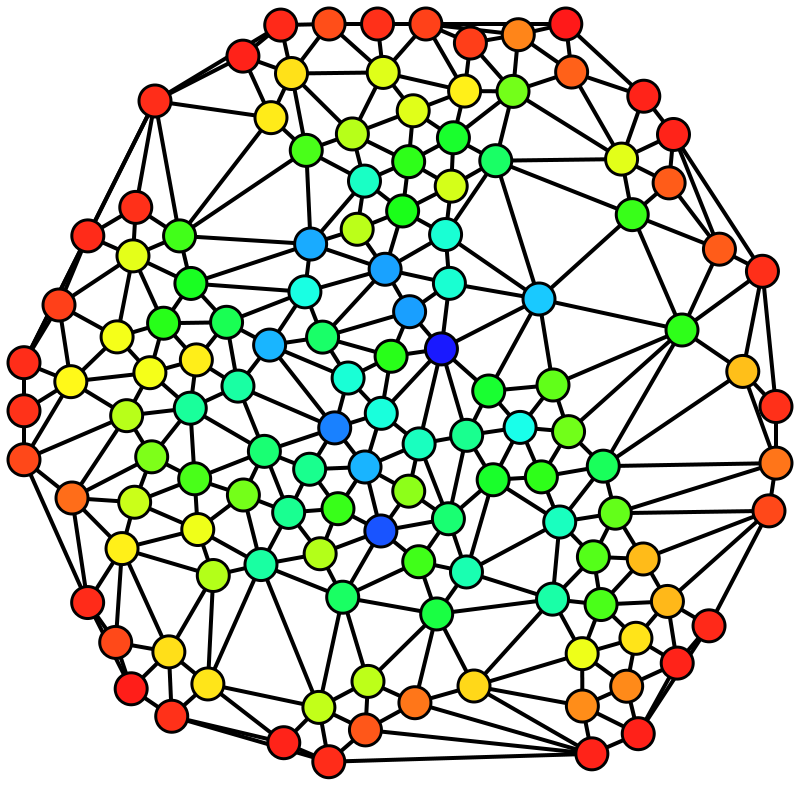
\includegraphics[width=42mm]{fig/Graph_betweenness.png}
\\ \hspace{10mm} \tiny{Example retrieved from  Wikipedia}
    \end{column}
  \end{columns}
}

%---------------------------------------------------------------------- SLIDE -
\frame{
\frametitle{Betweenness centrality}
\begin{itemize}
  \item Can be defined also for edges (similarly to nodes)
  \item Edges with high betweenness are what the sociologists call \emph{``weak ties''}. They tends to be the \emph{bridge} between two communities.
\end{itemize}

   \begin{columns}[T]
\begin{column}{60mm}
\emph{The strength of weak ties (Granovetter 1973)}
\begin{small}
\begin{itemize}
\item Dissemination and coordination dynamics are influenced by links established to nodes of different communities.
\item The importance of these links has become more and more with the rise of social networks and professional networking platforms.
\end{itemize}
\end{small}
   \end{column}
  \hspace{-16mm}\begin{column}{40mm}
 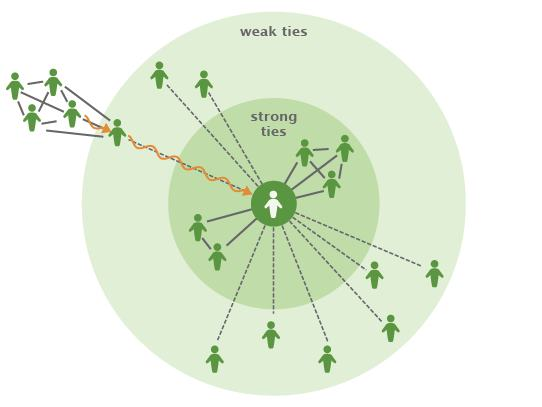
\includegraphics[width=62mm]{fig/weak_ties.png}
    \end{column}
  \end{columns}
}

%---------------------------------------------------------------------- SLIDE -
\frame{
\frametitle{Weak ties}
(Bakshy et al. 2012)
\begin{itemize}
\item
Weak links have a greater potential to expose links to new  contacts that otherwise would not have been discovered.
\end{itemize}

\begin{center}
 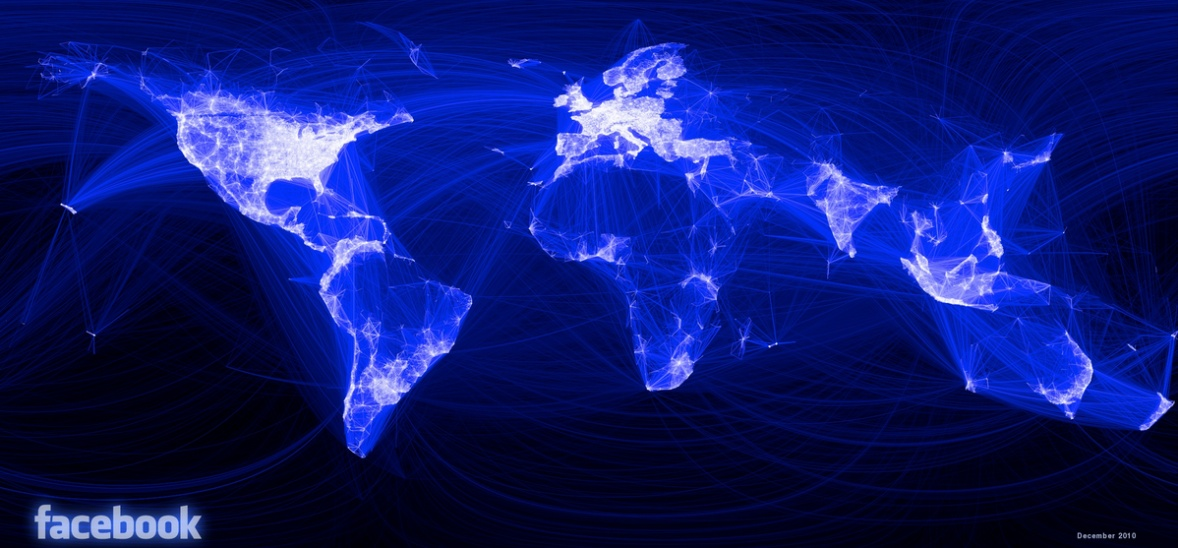
\includegraphics[width=70mm]{fig/facebook_graph.png}
 \end{center}
}

%---------------------------------------------------------------------- SLIDE -
\frame{
\frametitle{Weak ties}
(Grabowicz et al. 2012)
\begin{itemize}
\item Personal interactions are more likely to occur in internal links within communities (strong links)
 \item Events or new information is propagated faster by intermediate links (weak links).
\end{itemize}

\medskip

 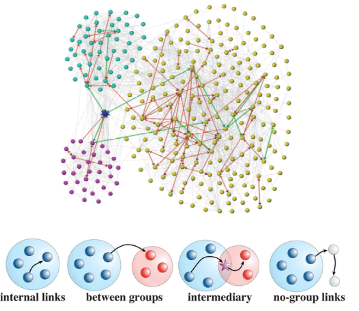
\includegraphics[width=50mm]{fig/weak_ties2.png}
 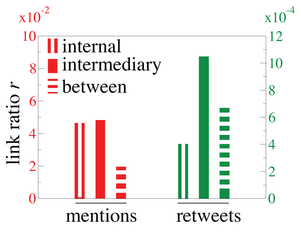
\includegraphics[width=50mm]{fig/weak_ties3.png}
}

%---------------------------------------------------------------------- SLIDE -
\frame{
\frametitle{Girvan-Newman algorithm for community detection (Girvan and Newman 2002)}
Hierarchical divisive clustering obtained by \emph{recursively removing the ``weakest tie''}.

\begin{enumerate}
  \item Compute edge betweenness centrality of all edges;
  \item Remove the edge with the highest betweenness centrality;
  \item Repeat from 1.
\end{enumerate}

\medskip
\centering
 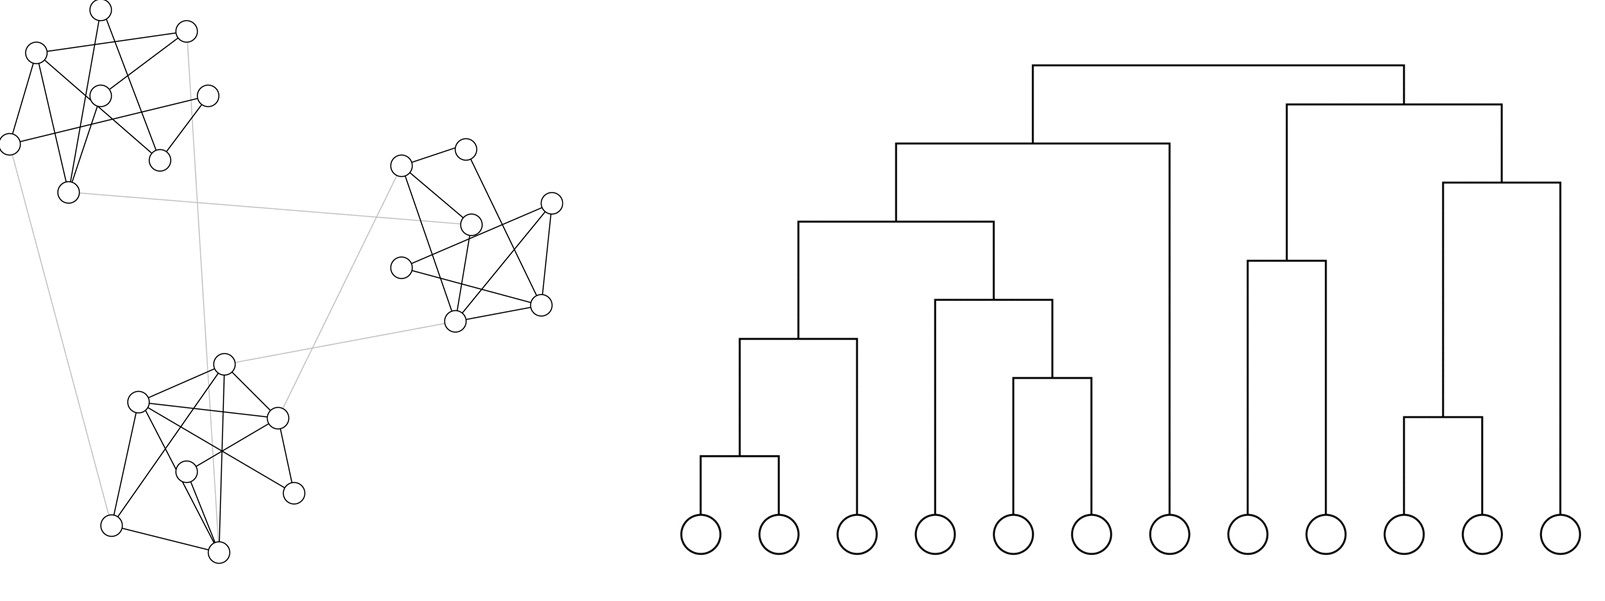
\includegraphics[width=82mm]{fig/gn.png}
}




%---------------------------------------------------------------------- SLIDE -
\frame{
\frametitle{Comparison}
\begin{block}{Which node is the most central?}
 \begin{itemize}
 \item for Degree Centrality:
 \item for Closeness Centrality:
 \item for Betweenness Centrality:
\end{itemize}
\end{block}
\centering
   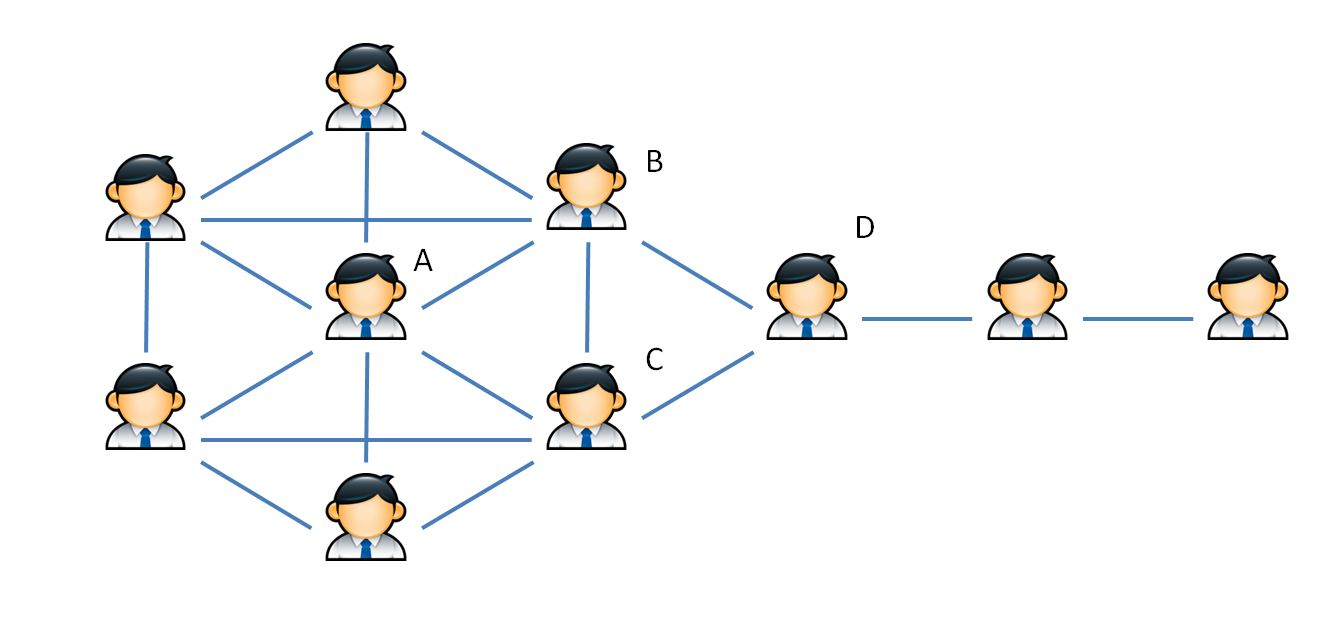
\includegraphics[width=100mm]{fig/centrality_comparison.png}
}

\frame{
\frametitle{Comparison}
\begin{block}{Which node is the most central?}
 \begin{itemize}
 \item for Degree Centrality:  {\color{blue}  user A}
 \item for Closeness Centrality:
 \item for Betweenness Centrality:
\end{itemize}
\end{block}
\centering
   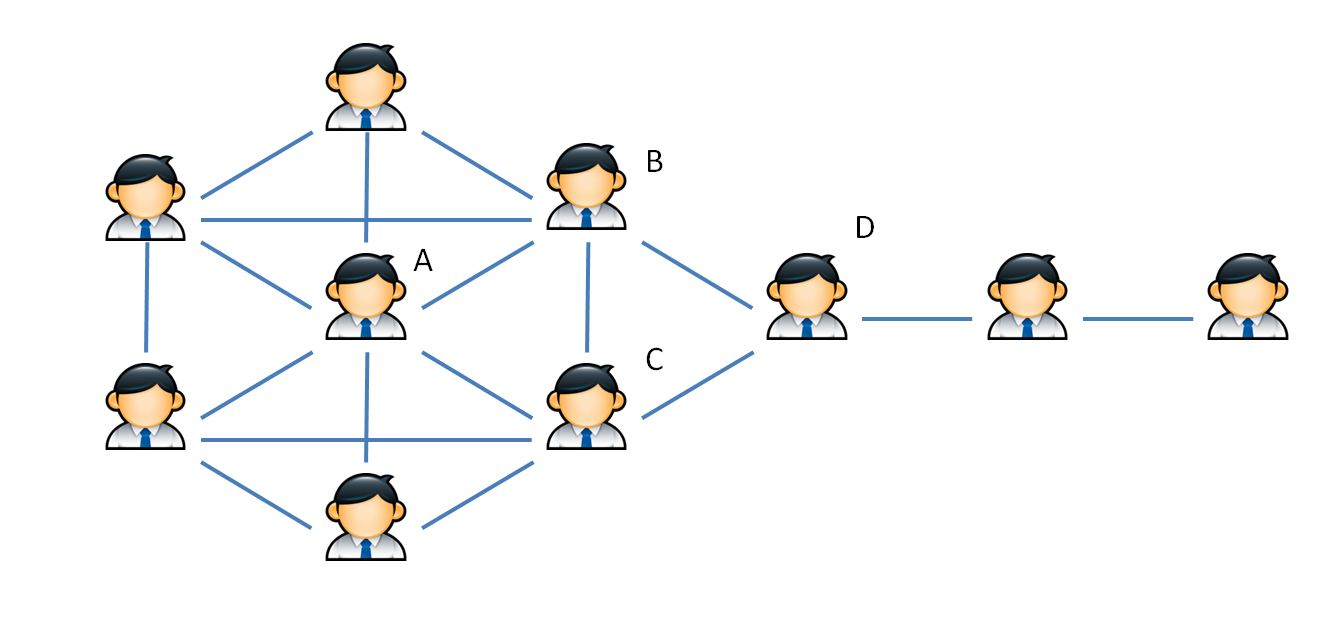
\includegraphics[width=100mm]{fig/centrality_comparison.png}
}

\frame{
\frametitle{Comparison}
\begin{block}{Which node is the most central?}
 \begin{itemize}
 \item for Degree Centrality: {\color{blue}  user A}
 \item for Closeness Centrality: {\color{blue}  users B and C}
 \item for Betweenness Centrality:
\end{itemize}
\end{block}
\centering
   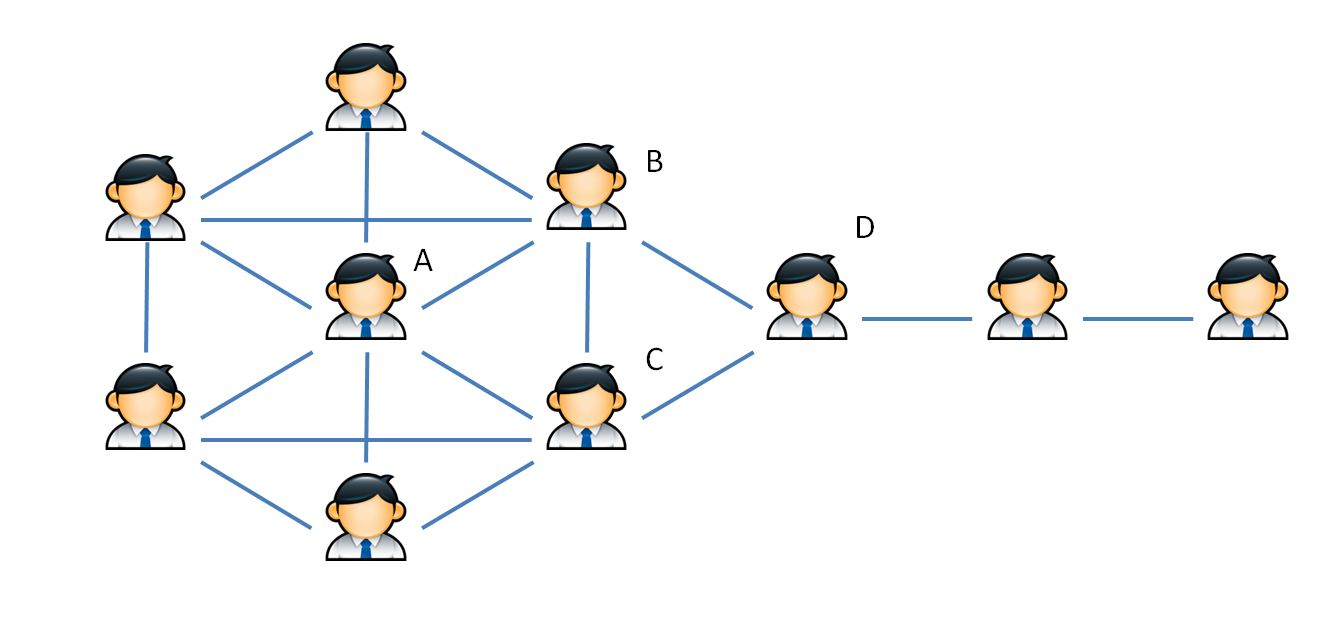
\includegraphics[width=100mm]{fig/centrality_comparison.png}
}

\frame{
\frametitle{Comparison}
\begin{block}{Which node is the most central?}
 \begin{itemize}
 \item for Degree Centrality: {\color{blue}  user A}
 \item for Closeness Centrality: {\color{blue}  users B and C}
 \item for Betweenness Centrality: {\color{blue}  user D}
\end{itemize}
\end{block}
\centering
   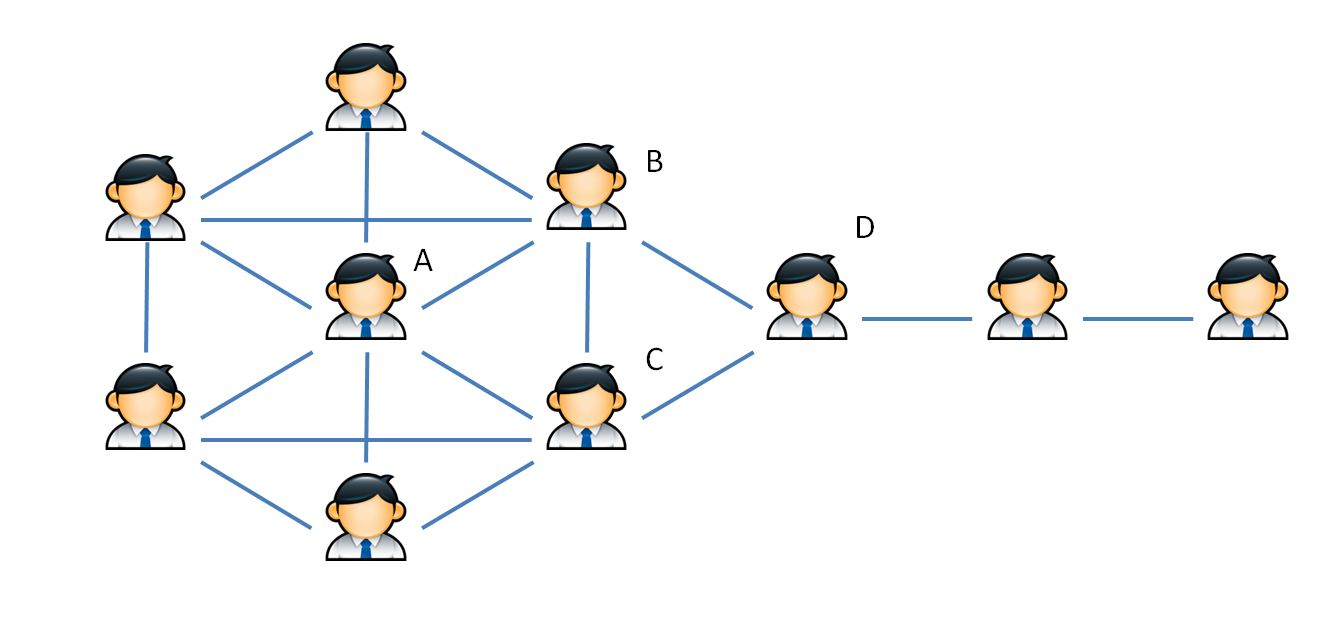
\includegraphics[width=100mm]{fig/centrality_comparison.png}
}

%---------------------------------------------------------------------- SLIDE -
\frame{
\frametitle{Visual Comparison}
 \begin{itemize}
 \item[A] Degree Centrality
 \item[B] Closeness Centrality
 \item[C] Betweenness Centrality
\end{itemize}

\centering
   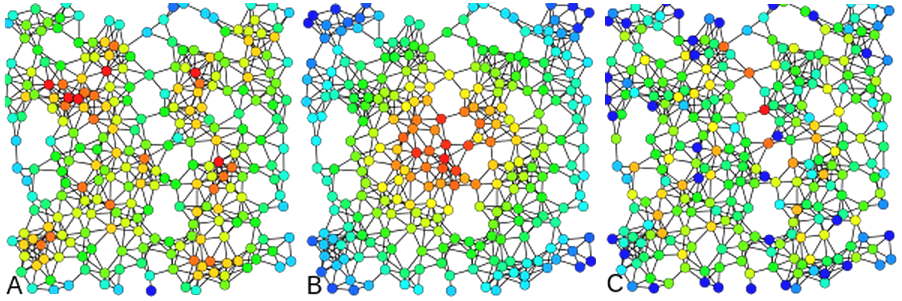
\includegraphics[width=100mm]{fig/centrality.png}
}




%---------------------------------------------------------------------- SLIDE -
\section{Axioms for centrality (Boldi and Vigna 2013)}




%---------------------------------------------------------------------- SLIDE -
\frame{
  \frametitle{Assessing}
  Is there a robust way to convince oneself that a certain centrality measure is
  better than another?

  Axiomatization\dots
  \begin{itemize}
    \pause\item \dots hard axioms (characterize a centrality measure completely)
    \pause\item \dots soft axioms (like the $T_i$ axioms for topological spaces)
  \end{itemize}
}

%---------------------------------------------------------------------- SLIDE -
\frame{
  \frametitle{Sensitivity to size}
  Idea: size matters!

   $S_{k,p}$ be the union of a $k$-clique and a $p$-cycle.
  \begin{itemize}
   \item if $k\to\infty$, every node of the clique becomes ultimately
    strictly more important than every node of the cycle
  \item if $p\to\infty$, every node of the cycle becomes ultimately
    strictly more important than every node of the clique
  \end{itemize}

  \medskip
  \centering
 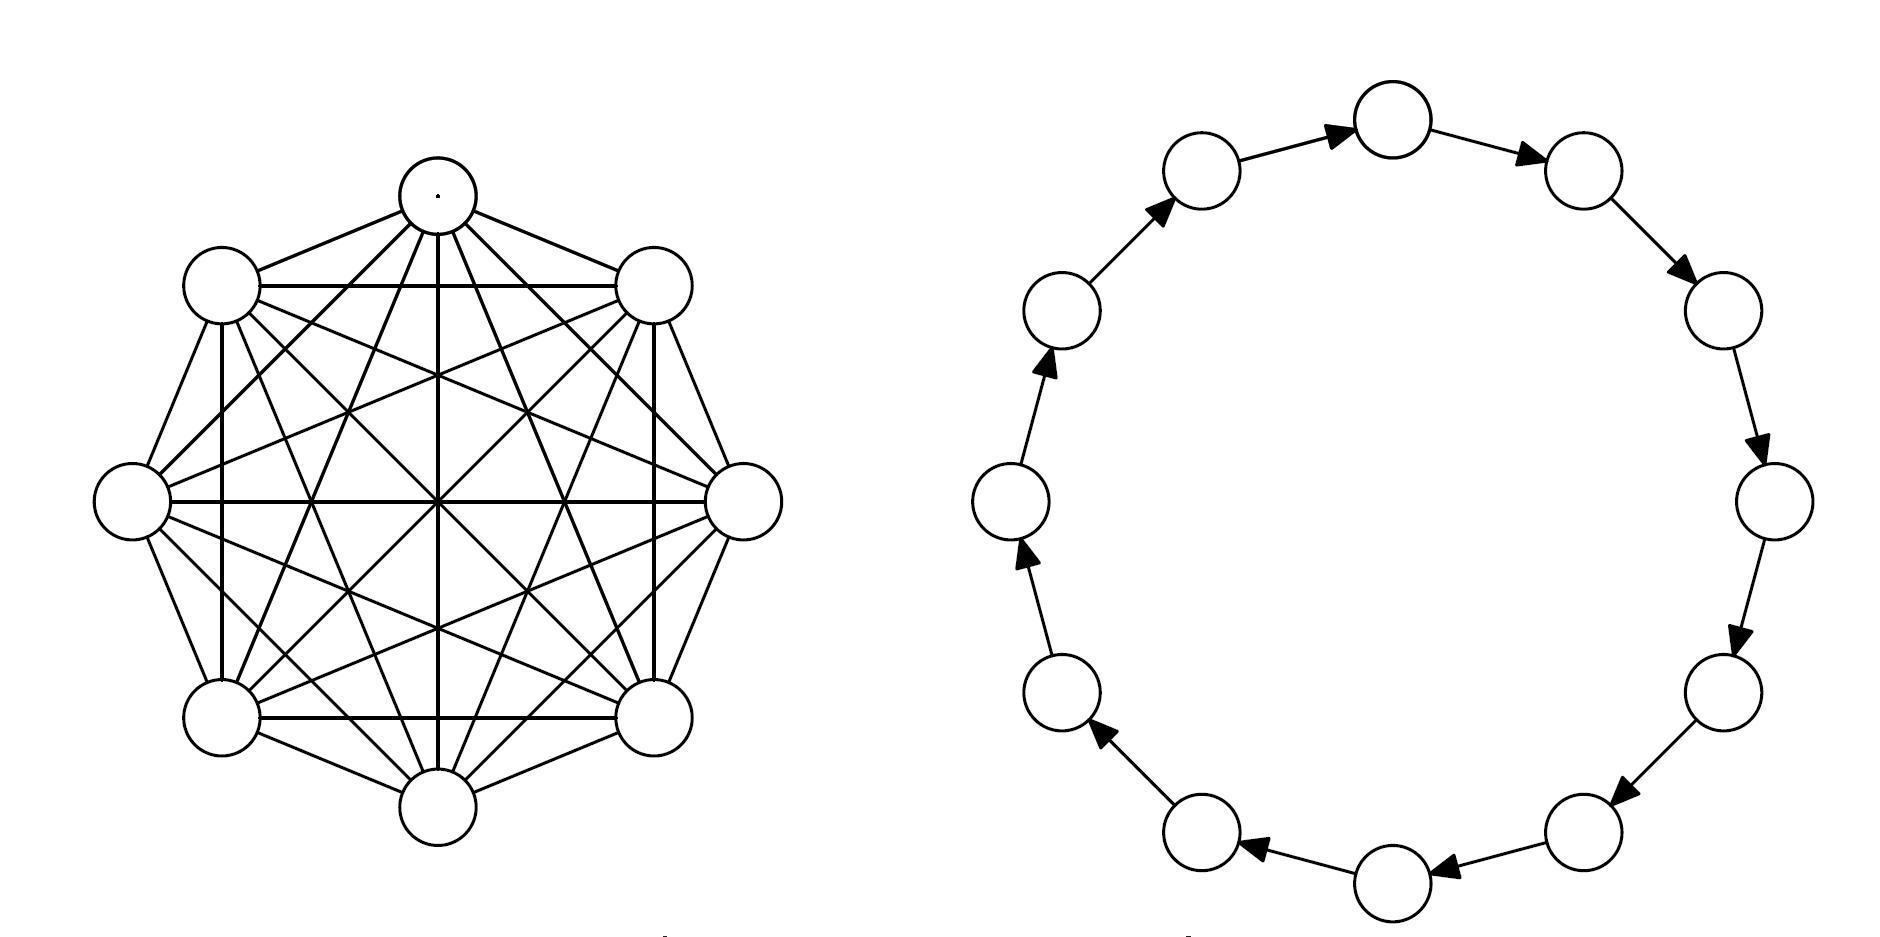
\includegraphics[width=82mm]{fig/sts.png}
}

%---------------------------------------------------------------------- SLIDE -
\frame{
  \frametitle{Sensitivity to density}
  Idea: density matters!

 $D_{k,p}$ be made by a $k$-clique and a $p$-cycle connected by a single
  bidirectional bridge:
  \begin{itemize}
    \item if $k\to\infty$, the node on the clique-side of the bridge
    becomes more important than the node on the cycle-side.
  \end{itemize}

    \medskip
  \centering
 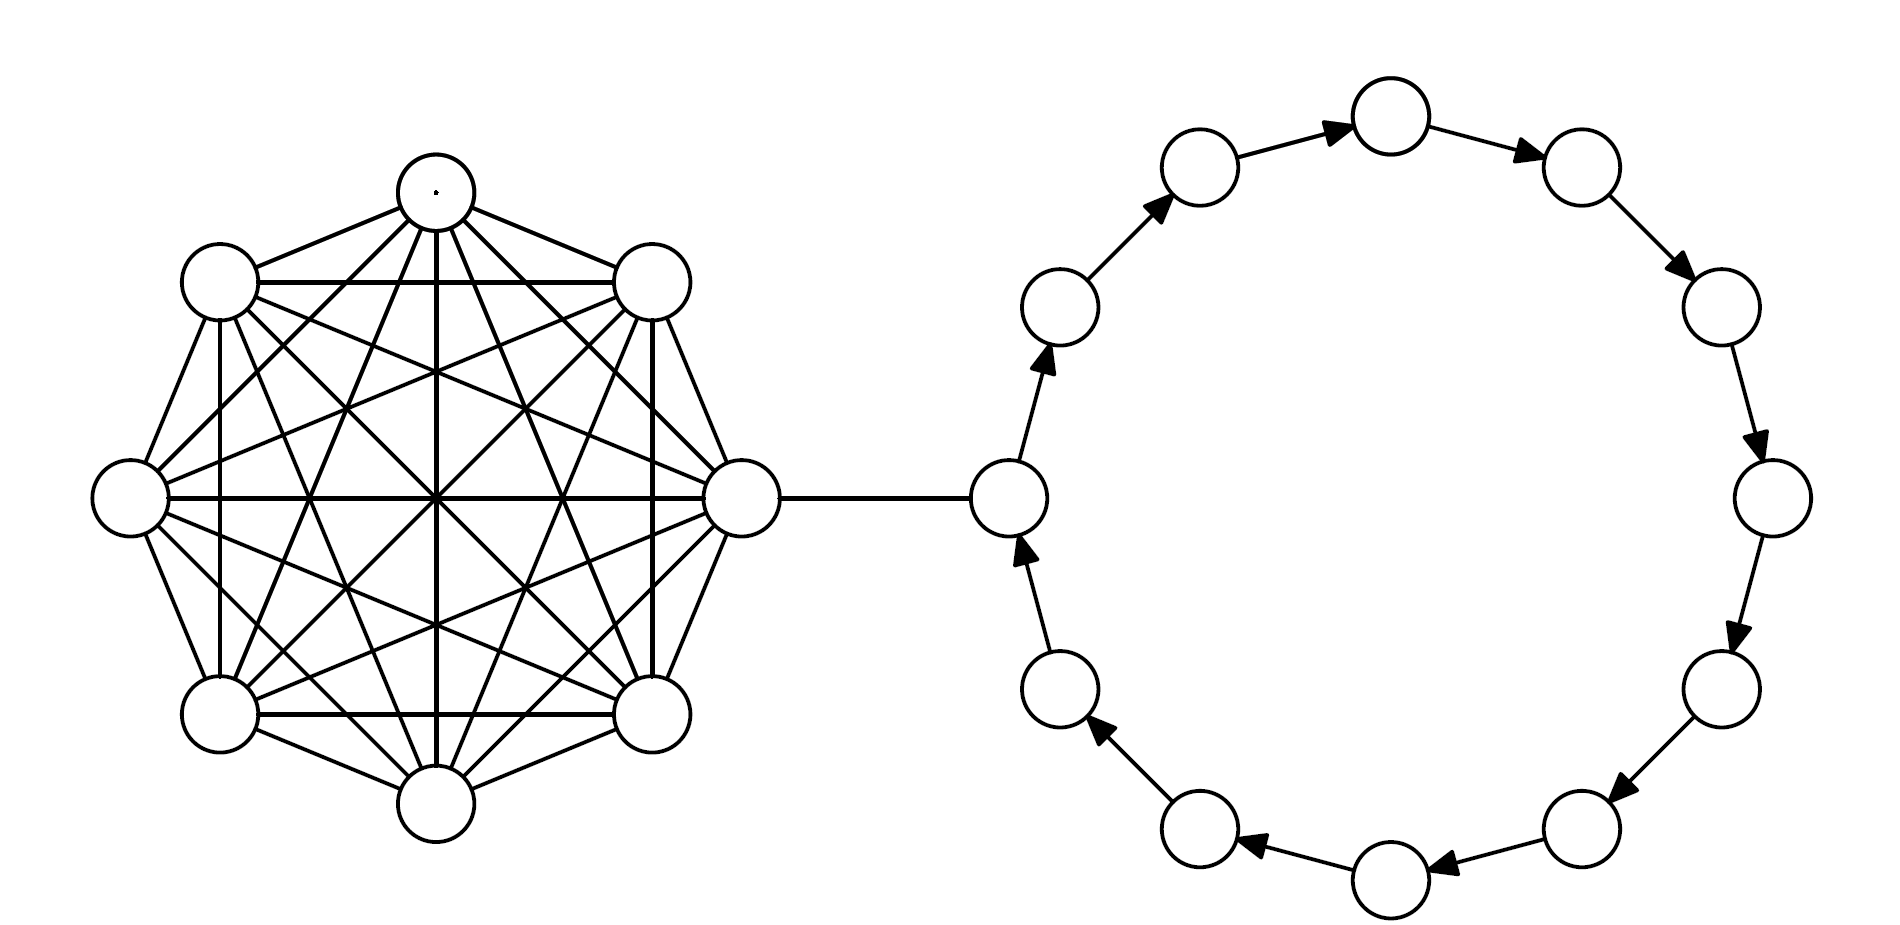
\includegraphics[width=82mm]{fig/std.png}
}

%---------------------------------------------------------------------- SLIDE -
\frame{
  \frametitle{Score monotonicity}
  Adding an arc $x \to y$ strictly increases the score of $y$.

  \smallskip
  \pause {\bf Doesn't say anything about the score of other nodes!}
}

%---------------------------------------------------------------------- SLIDE -
\frame{
  \frametitle{Rank monotonicity}
  Adding an arc $x \to y$\dots
  \begin{itemize}
    \pause\item if $y$ used to dominate $z$, then the same holds after adding
    the arc
    \pause\item if $y$ had the same score as $z$, then the same holds after
    adding the arc
	\pause\item {\bf strict variant: } if $y$ had the same score as $z$, then $y$
	dominates $z$ after adding the arc
  \end{itemize}
}

%---------------------------------------------------------------------- SLIDE -
\frame{
  \frametitle{Rank monotonicity}
\begin{table}
\renewcommand{\arraystretch}{1.2}
\begin{minipage}{\textwidth}
\centering
\begin{tabular}{l|c|c|c|c|c|c}
\multicolumn{1}{c|}{}&\multicolumn{4}{c|}{Monotonicity}&\multicolumn{2}{c}{Other axioms}\\
\multicolumn{1}{c|}{}&\multicolumn{2}{c|}{General}&\multicolumn{2}{c|}{Strongly connected}&\multicolumn{2}{c}{}\\
Centrality & Score & Rank & Score & Rank & Size & Density
\\
\hline
Harmonic & yes  & yes* & yes & yes* & yes & yes \\
Degree  & yes & yes* & yes & yes* & only $k$ & yes \\
Katz & yes & yes*& yes & yes* & only $k$ & yes \\
PageRank &  yes & yes*& yes & yes* & no & yes \\
Seeley & no & no & yes & yes & no & yes \\
Closeness & no  & no & yes & yes & no & no \\
Lin & no & no & yes & yes & only $k$& no \\
Betweenness & no & no & no & no & only $p$ & no \\
Dominant & no & no &? &? & only $k$ & yes \\
HITS & no & no & no &no & only $k$ &yes\\
SALSA & no & no & no &no & no & yes
\end{tabular}
\end{minipage}
\end{table}
}

%---------------------------------------------------------------------- SLIDE -
\frame{
  \frametitle{Kendall's $\tau$}

\begin{tabular}{c}
  Hollywood collaboration network\\
 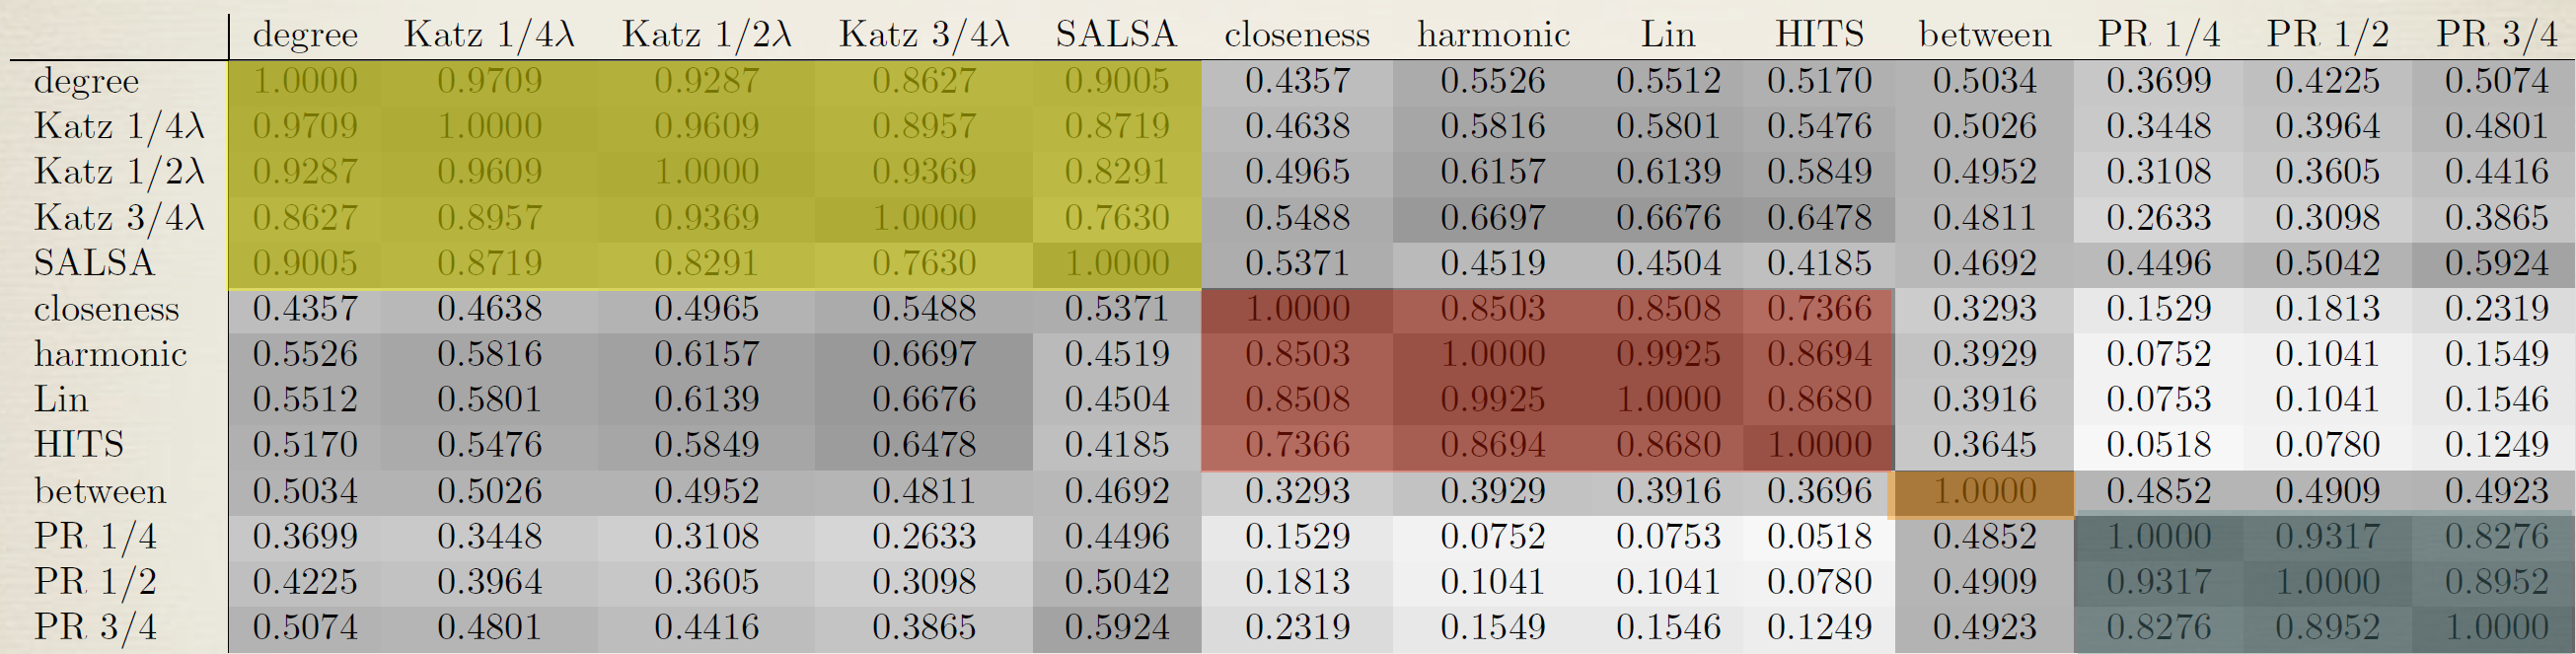
\includegraphics[width=\textwidth]{fig/kendall2.png}\\
 \medskip \\
  .uk (May 2007 snapshot)\\
 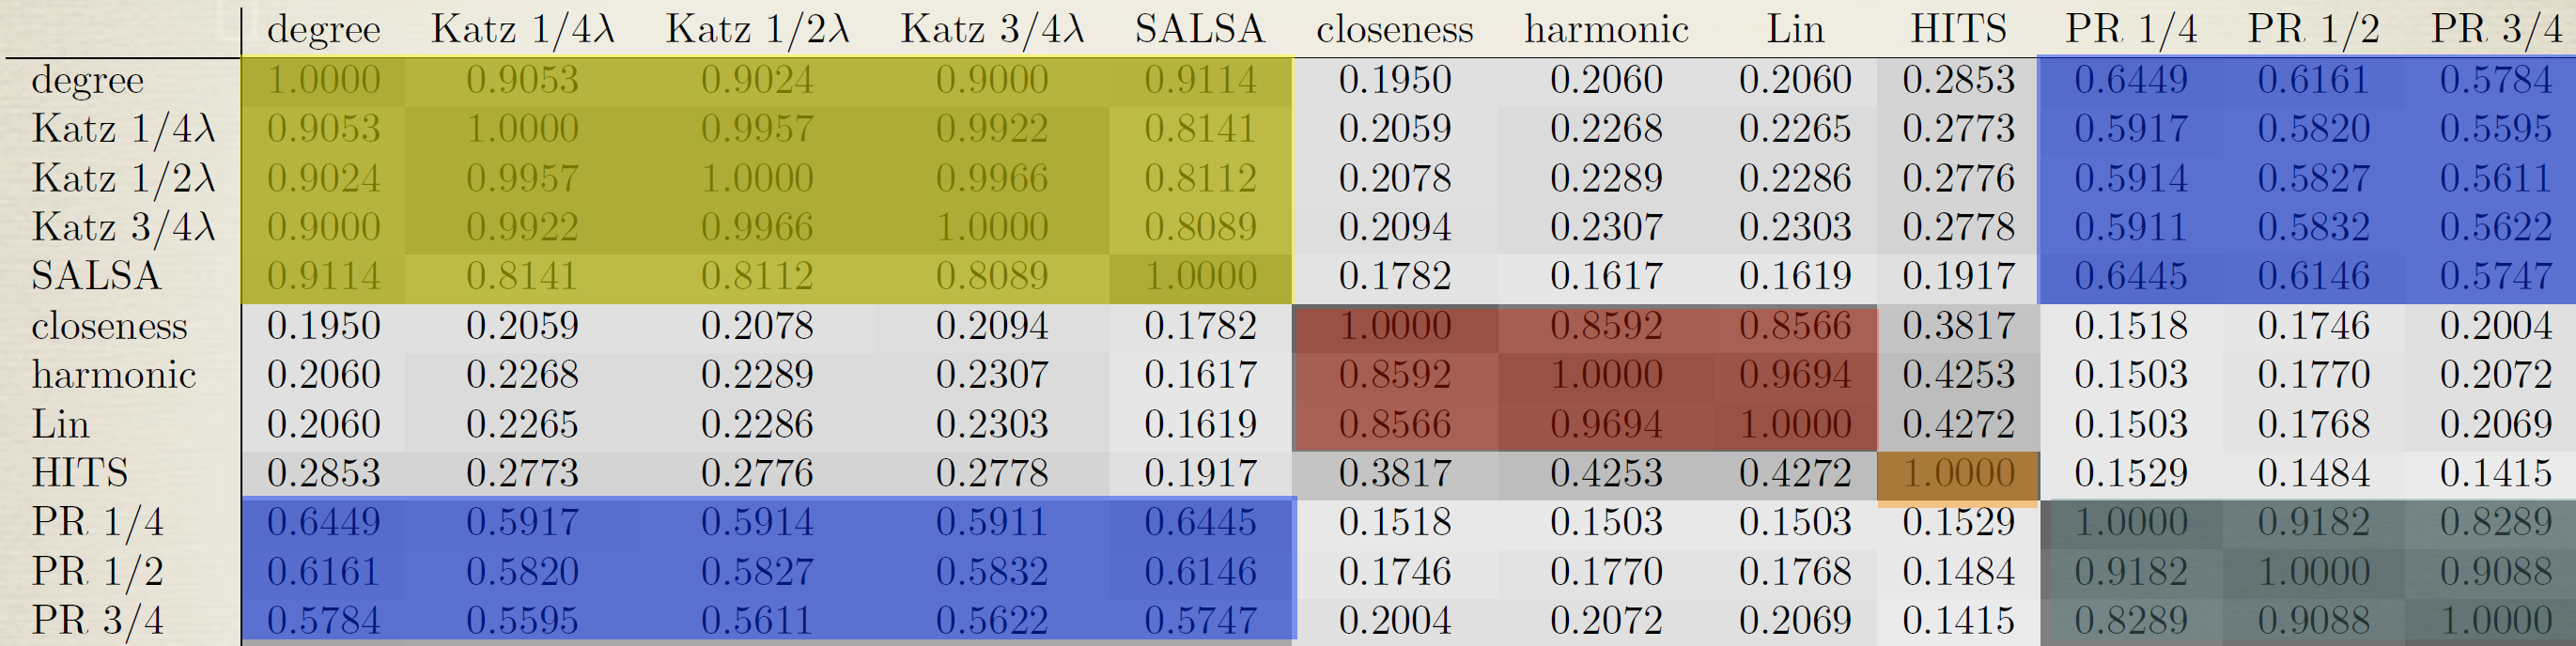
\includegraphics[width=\textwidth]{fig/kendal.png}\\
\end{tabular}
}

%---------------------------------------------------------------------- SLIDE -
\frame{
  \frametitle{Correlation}
\begin{itemize}
 \pause \item most geometric indices and HITS
are rather correlated to one another;
  \pause \item Katz, degree and SALSA are also
highly correlated;
  \pause \item PageRank stands alone in the first dataset, but it is correlated to degree, Katz, and SALSA in the second dataset;
  \pause \item Betweenness is not correlated to anything in the first dataset, and could not be computed in the second dataset due to the size of the graph (106M vertices).
\end{itemize}

}



\begin{frame}
  \frametitle{What vertices in a graph are important?}
  Betweenness centrality is one measure of vertex importance\\
  \quad Roughly, it is the fraction of Shortest Paths (SP) in a graph that go through a vertex
  \vfill
  Let $G=(V,E)$, $|V|=n$, $|E|=m$. The betweenness centrality of $v\in V$ is:
  \[
    \betw(v)=\underbrace{\frac{1}{n(n-1)}}_{\mbox{normalization}}\sum_{p_{uw}\in\mathbb{S}_G}
    \underbrace{\frac{\mathds{1}_{\mathcal{T}_v}(p_{uw})}{\sigma_{uw}}}_{\in [0,1]}
  \]
  where:
  \begin{itemize*}
    \item $\mathbb{S}_G$: set of all SPs in $G$
    \item $\mathcal{S}_{uw}$: set of all SPs from $u$ to $w$
      ($\mathcal{S}_{uw}\subseteq\mathbb{S}_G$,
      $|\mathcal{S}_{uw}|=\sigma_{uw}$)
    \item $\mathcal{T}_v$: $\{p\in\mathbb{S}_G ~:~ v\in\mathsf{Int}(p)\}$
  \end{itemize*}
\end{frame}

\begin{frame}
  \frametitle{How to compute betweenness centrality?}
  Na\"ive algorithm: All Pairs SP computation, followed by aggregation\\
  \quad Aggregation dominates runtime, $\Theta(n^3)$
  \vfill
  [Brandes 2001]: Perform aggregation after each Single-Source SP (SSSP) computation\\
  \quad Runtime: $O(nm)$ (unweighted $G$), $O(nm + n^2\log n)$ (weighted
  $G$)\\
  This is is still too much for graphs with $n=10^9$, $m=10^10$
  \vfill
  Possible solution: perform fewer SPs computations by sampling\\
  \quad We get approximate results, but that's OK!
  \vfill
  What kind of approximation do we want ? What should we sample and how much?
\end{frame}

\begin{frame}
  \frametitle{What kind of approximation do we want?}
  We want uniform quality guarantees on the approximations of all vertices
  \vfill
  Definition:\\
  \quad For $\varepsilon,\delta\in(0,1)$, an $(\varepsilon,\delta)$-approximation is
  a collection $\{\tilde{\betw}(v), v\in V\}$ such that
  \[
    \Pr(\exists v\in V ~:~ |\tilde{\betw}(v) -\betw(v)|>\varepsilon)<\delta
  \]
  $\varepsilon$ controls the accuracy, $\delta$ controls the confidence
  \vfill
  Trade-off: smaller $\varepsilon$ or $\delta$ $\Rightarrow$ higher number of
  samples $\Rightarrow$ slower runtime
\end{frame}

\begin{frame}
  \frametitle{How can one get an $(\varepsilon,\delta)$-approximation?}
  [Brandes and Pich, 2008]: only run SSSP and aggregation from a few sources
  \vfill
  \begin{algorithm}[H]
    \DontPrintSemicolon
    $r\leftarrow \frac{1}{\varepsilon^2}\left(\ln n + \ln 2 +
    \ln\frac{1}{\delta}\right)$ \texttt{// sample size}\;
    $\tilde{\betw}(v)\leftarrow 0$, for all $v\in V$\;
    \For(\texttt{// the exact algorithm would iterate over $V$}){$i\leftarrow 1,\dotsc,r$} {
      $v_i \leftarrow$ random vertex from $V$, chosen uniformly\;
      Perform single-source SP computation from $v_i$\;
      Perform partial aggregation, updating $\tilde{\betw}(u)$, $u\in V$,
      like in exact algorithm\;
    }
    Output $\{\tilde{\betw{v}}, v\in V\}$\;
  \end{algorithm}
  \vfill
  Theorem: The output is an $(\varepsilon,\delta)$-approximation
\end{frame}

\begin{frame}
  \frametitle{How do they prove it?}
  Start with bounding the deviation for a single vertex $v$ (Hoeffding bound):
  \[
    \Pr(|\tilde{\betw}(v)-\betw(v)|>\varepsilon)\le 2e^{-2r\varepsilon^2}
  \]
  \vfill
  Then take the union bound over $n$ vertices to ensure uniform converge\\
  \quad the sample size $r$ must be such that
  \[
    2e^{-2r\varepsilon^2}\le\frac{\delta}{n}
  \]
  That is, to get an $(\varepsilon,\delta)$-approximation, we need
  \[
    r\ge\frac{1}{2\varepsilon^2}\left(\ln n + \ln 2 +
    \ln\frac{1}{\delta}\right)
  \]
\end{frame}

\begin{frame}
  \frametitle{What is wrong with this approach?}
  1) We need
  \[
    r\ge\frac{1}{2\varepsilon^2}\left(\ln n + \ln 2 +
    \ln\frac{1}{\delta}\right)
  \]
  \begin{itemize}
    \item This is loose, due to the union bound and does not scale well (experiments)
    \item The sample size depends on $\ln n$. This is not the right
      quantity: not all graphs of $n$ nodes are equally ``difficult'': e.g., the $n$-star is ``easier'' than a random graph
  \end{itemize}
  The sample size $r$ should depend on a more-specific characteristic of the graph
  \vfill
  2) At each iteration, the algorithm performs a SSSP computation\\
  \quad Full exploration of the graph, no locality
\end{frame}

\begin{frame}
  \frametitle{How can we improve the sample size?}
  [R. and Kornaropoulos, 2014] present an algorithm that:
  \vfill
  1) uses a sample size which depends on the vertex-diameter, a characteristic
  quantity of the graph. The derivation uses VC-dimension
  \vfill
  2) samples SPs according to a specific, non-uniform distribution over
  $\mathbb{S}_G$. For each sample, it performs a single $s-t$ SP computation
    \begin{itemize}
      \item More locality: fewer edges touched than single-source SP
      \item Can use bidirectional search / A\textsuperscript{*},
        \ldots
      \end{itemize}
\end{frame}

\begin{frame}
  \frametitle{What is the algorithm?}
  \begin{algorithm}[H]
    \DontPrintSemicolon
    $\mathsf{VD}(G)\leftarrow$ vertex-diameter of $G$ \texttt{// stay
    tuned!}\;
    $r\leftarrow\frac{1}{2\varepsilon^2}\left(\lfloor\log_2(\mathsf{VD}(G)-2\rfloor)
    +1 + \ln(1/\delta)\right)$ \texttt{// sample size}\;
    $\tilde{\betw}(v)\leftarrow 0$, for all $v\in V$\;
    \For{$i\leftarrow 1\dotsc,r$}{
      $(u,v)\leftarrow$ random pair of different vertices, chosen
      uniformly\;
      $\mathcal{S}_{uv}\leftarrow$ all SPs from $u$ to $v$ \texttt{//
      Dijkstra, trunc.~BFS, \ldots}\;
      $p\leftarrow$ random element of $\mathcal{S}_{uv}$, chosen
      uniformly \texttt{// not uniform over $\mathbb{S}_G$}\;
      $\tilde{\betw}(w)\leftarrow \tilde{\betw}(w) + 1/r$, for all
      $w\in\mathsf{Int}(p)$ \texttt{// update only nodes along $p$}\;
    }
    Output $\{\tilde{\betw}(v), v\in V\}$
  \end{algorithm}
  Theorem: The output $\{\tilde{\betw}(v), v\in V\}$ is an
  $(\varepsilon,\delta$)-approximation
\end{frame}

\begin{frame}
  \frametitle{How can we prove the correctness?}
  We want to prove that the output $\{\tilde{\betw}(v), v\in V\}$ is an
  $(\varepsilon,\delta$)-approximation
  \vfill
  Let's apply the recipe!

  \begin{enumerate}
    \item  Define betweenness centrality computation as a expectation
      estimation problem (domain $\domain$, family $\family$, distribution
      $\prob$)
    \item Show that the algorithm efficiently samples according to $\prob$
    \item Show how to efficiently compute an upper bound to the VC-dimension\\
      \quad Bonus: show tightness of bound
    \item Apply the VC-dimension sampling theorem
  \end{enumerate}
\end{frame}

\begin{frame}
  \frametitle{How to define the expectation estimation task?}
  \begin{itemize}
    \item The domain $\domain$ is $\mathbb{S}_G$ (all SPs in $G$)\\
    \item The family is $\family=\{\mathds{1}_{\mathcal{T}_v}, v\in V\}$,
      where $\mathcal{T}_v=\{p\in\mathbb{S}_G ~:~: v\in\mathsf{Int}(p)\}$
    \item The probability distribution $\prob$ on $\domain$ is
      \[
        \pi(p_{uw})=\frac{1}{n(n-1)}\frac{1}{\sigma_{uw}}
      \]
      The algorithm samples paths according to $\pi$
  \end{itemize}
  \vfill
  We have
  \[
    \expectation_\pi[\mathds{1}_{\mathcal{T}_v}]=\sum_{p_{uw}\in\mathbb{S}_G}\mathds{1}_{\mathcal{T}_v}\pi(p_{uw})=\sum_{p_{uw}\in\mathbb{S}_G}\mathds{1}_{\mathcal{T}_v}(p_{uw})\frac{1}{n(n-1)}\frac{1}{\sigma_{uw}}=\betw(v)
  \]
\end{frame}

\begin{frame}
  \frametitle{How do we bound the VC-dimension?}
  Definition: The vertex-diameter $\mathsf{VD}(G)$ of $G$ is the maximum
  number of vertices in a SP of $G$
  \[
    \mathsf{VD}(G)=\max\{|p|, p\in\mathbb{S}_G\}
  \]
  If $G$ is unweighted, $\mathsf{VD}(G)=\Delta(G)+1$. Otherwise no relationship\\
  Very small in social networks, even huge ones (shrinking diameter effect)
  \vfill
  Computing $\mathsf{VD}(G)$: $\left(2\frac{\mbox{max.~edge weight}}{\mbox{min.~edge
  weight}}\right)$-approximation via single-source SP
  \vfill
  Theorem: The VC-dimension of $(\mathbb{S}_G,F)$ is at most $\lfloor\log_2\mathsf{VD}(G)
  -2\rfloor +1$
\end{frame}

\begin{frame}
  \frametitle{Let's prove it!}
  Theorem: The VC-dimension is at most $\lfloor\log_2\mathsf{VD}(G)
  -2\rfloor +1$
  \vfill
  Proof:
  \begin{itemize}
    \item For a set $A\subseteq\mathbb{S}_G$ of size $|A|=d$ to be
      shattered, any $p$ in $A$ must appear in at least $2^{d-1}$
      different sets $\mathcal{T}_v$, one for each subset of $A$
      containing $p$.
    \item Any $p$ appears only in the sets $\mathcal{T}_v$ such that
      $v\in\mathsf{Int}(p)$\\
      \quad There are $|\mathsf{Int}(p)|$ such sets
    \item From the definition of the vertex-diameter $\mathsf{VD}(G)$, we have
      $|\mathsf{Int}(p)|\le\mathsf{VD}(G)-2$
    \item To shatter $A$, $d$ must be such that $2^{d-1}\le\mathsf{VD}(G)-2$
    \item So $d$ can be at most $\lfloor\log_2\mathsf{VD}(G) -2\rfloor +1$,
      otherwise $A$ can not be shattered
  \end{itemize}
\end{frame}

\begin{frame}
  \frametitle{How to use the bound?}
  We have that:
  \begin{itemize}
    \item The estimation $\tilde{\betw}(v)$ computed by the algorithm is the
      empirical average for $\betw(v)$
    \item The algorithm samples SPs efficiently according to $\prob$
    \item We know an upper bound to the VC-dimension and how to compute it
      efficiently
  \end{itemize}
  Thus we can apply the VC $\varepsilon$-sample theorem, and obtain that the algorithm
  outputs an $(\varepsilon,\delta)$-approximation:
  \[
    \Pr(\exists v\in V ~:~ |\tilde{\betw}(v)-\betw(v)|>\varepsilon)<\delta
  \]
\end{frame}

\begin{frame}
  \frametitle{Is the bound to the VC-dimension tight?}
  Yes! There is a class of graphs with VC-dimension exactly
  $\lfloor\log_2\mathsf{VD}(G) -2\rfloor +1$\\
  \quad The Concertina Graph Class $(G_i)_{i\in\mathbb{N}}$:
  \begin{figure}[H]
    \centering
    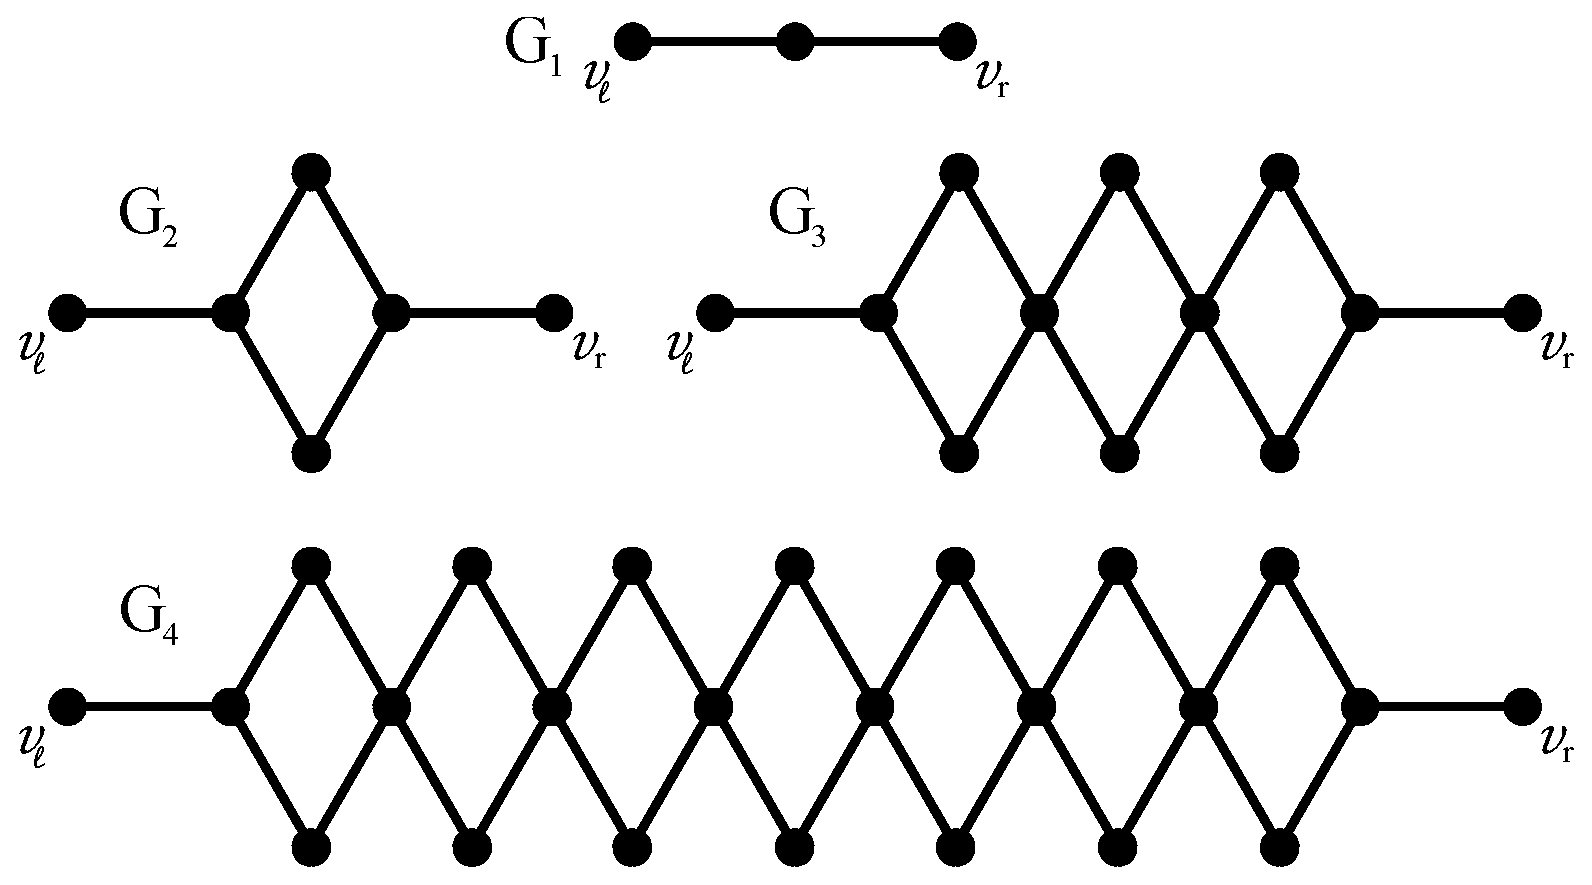
\includegraphics[scale=0.3]{figs/concertina}
  \end{figure}
  \vfill
  Theorem: The VC-dimension of $(\mathbb{S}_{G_i}, F)$ is
  $\lfloor\log_2\mathsf{VD}(G) -2\rfloor +1=i$
  \vfill
  Proof Intuition: The middle vertices are internal to a lot of SPs
\end{frame}

\begin{frame}
  \frametitle{Is the Vertex-Diameter the right quantity?}
  No! If $G$ undirected and for every connected pair of nodes there is a
  unique SP, then the VC-dimension is at most 3\\
  \quad These graphs are not just trees!
  \vfill
  Proof: in such a graph, two SPs that meet and separate can not meet again\\
  \quad (+ multiple case analysis)
  \vfill
  The bound ``3'' is tight. In the following graph we can shatter 3 paths
  \begin{figure}[H]
    \centering
    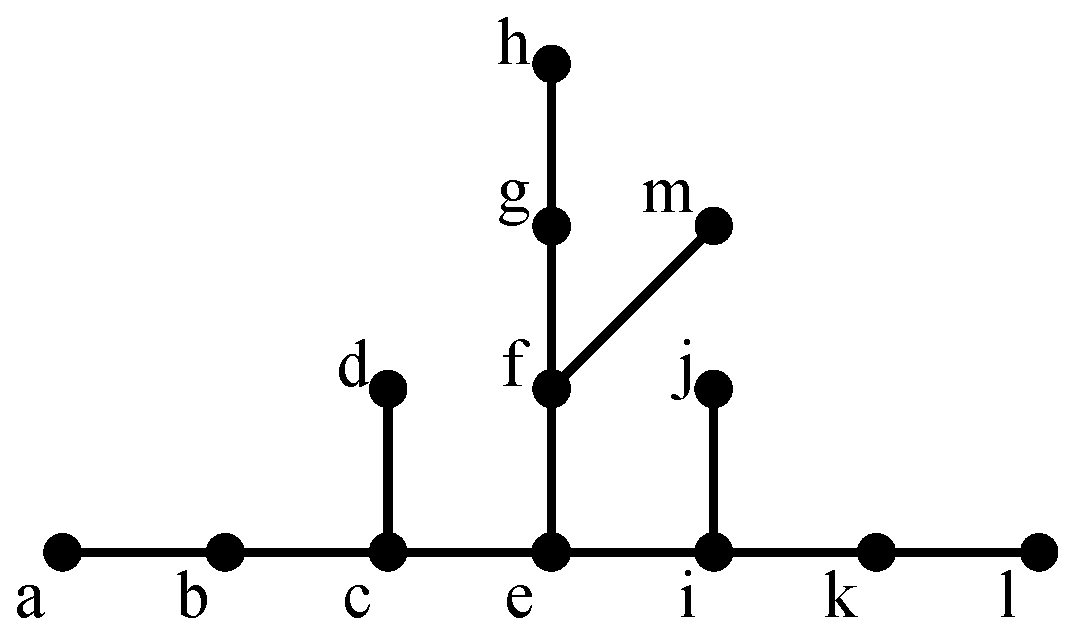
\includegraphics[scale=0.3]{figs/uniqueshortestpathtight}
  \end{figure}
  \vfill
  There is room for improvement using pseudodimension (we are working on that!)
\end{frame}

\begin{frame}
  \frametitle{What about directed graphs?}
  Does a similar result also hold for directed graphs with unique SP?\\
  \quad  Not for the same constant $3$. We built a graph with unique SPs between
  all connected nodes and we can shatter a set of $4$ SPs
  \begin{figure}[H]
    \centering
    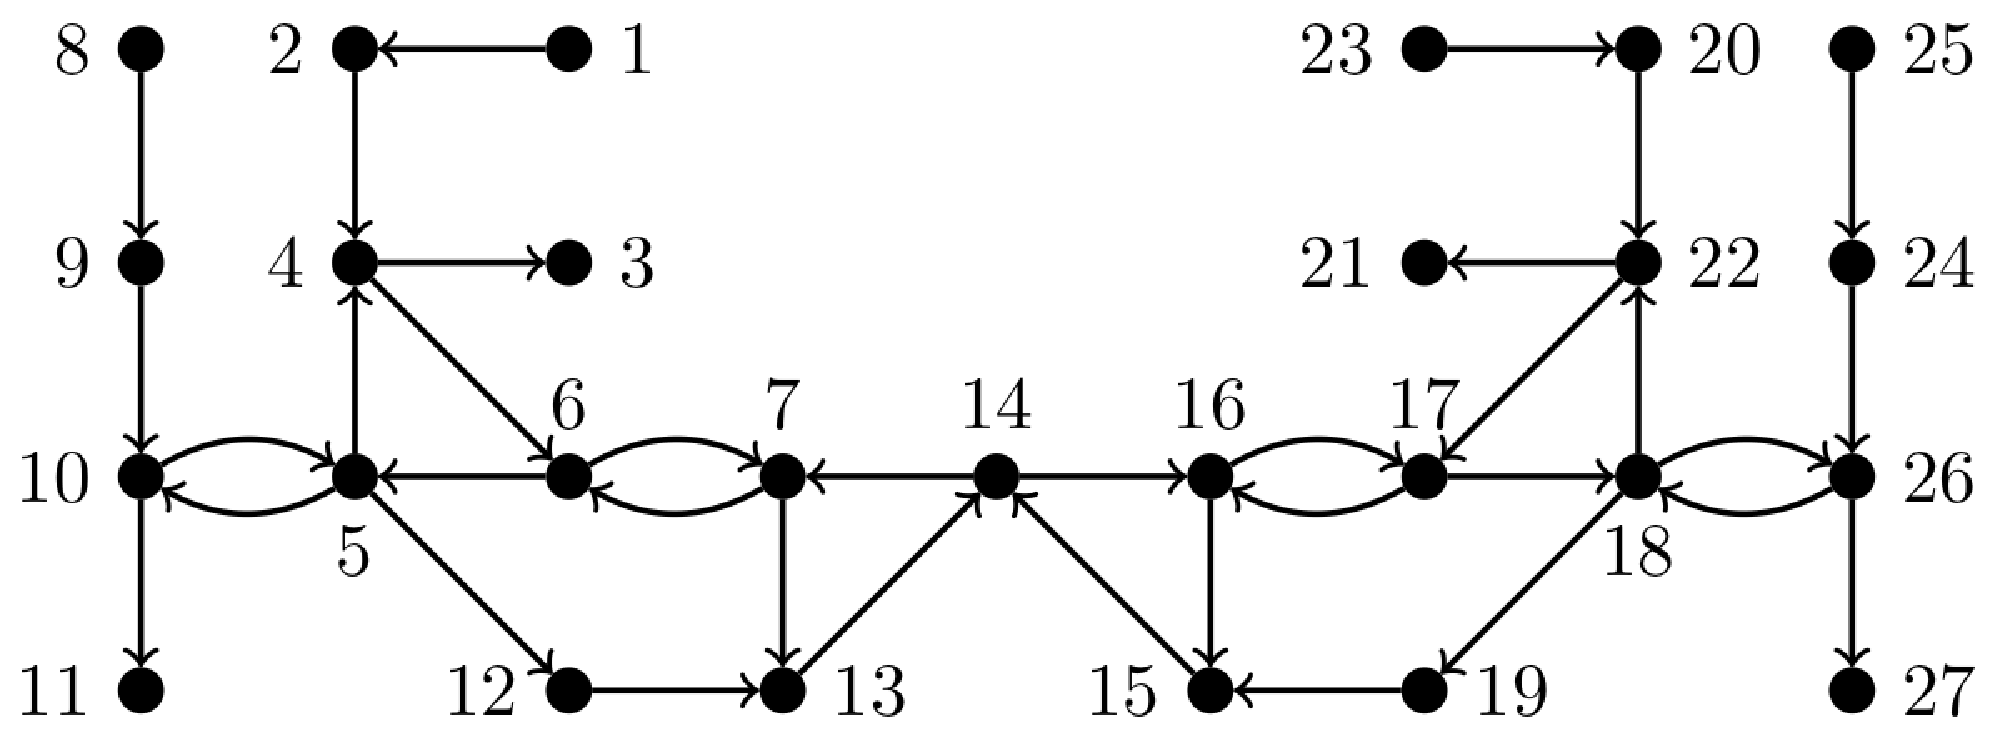
\includegraphics[scale=0.3]{figs/uniquedirected}
  \end{figure}
  Yes, finding counterexamples is messy\ldots
  \vfill
  Does it hold for a different constant?\\
  \quad We do not know! Maybe you can work on that?
\end{frame}

\begin{frame}
  \frametitle{How well does the algorithm perform in practice?}
  It performs very well!
  \vfill
  We tested the algorithm on real graphs (SNAP) and on artificial
  Barabasi-Albert graphs, to evalue its accuracy, speed, and scalability
  \vfill
  Results: It blows away the exact algorithm and the union-bound-based
  sampling algorithm
\end{frame}

\begin{frame}
  \frametitle{How accurate is the algorithm?}
  In $O(10^3)$ runs of the algorithm on different graphs and with different
  parameters, we always had $|\tilde{\betw}(v)-\betw(v)|<\varepsilon$ for all
  nodes\\
  \quad Actually, on average $|\tilde{\betw}(v)-\betw(v)|<\varepsilon/8$
  \vfill
  \begin{figure}[H]
    \centering
    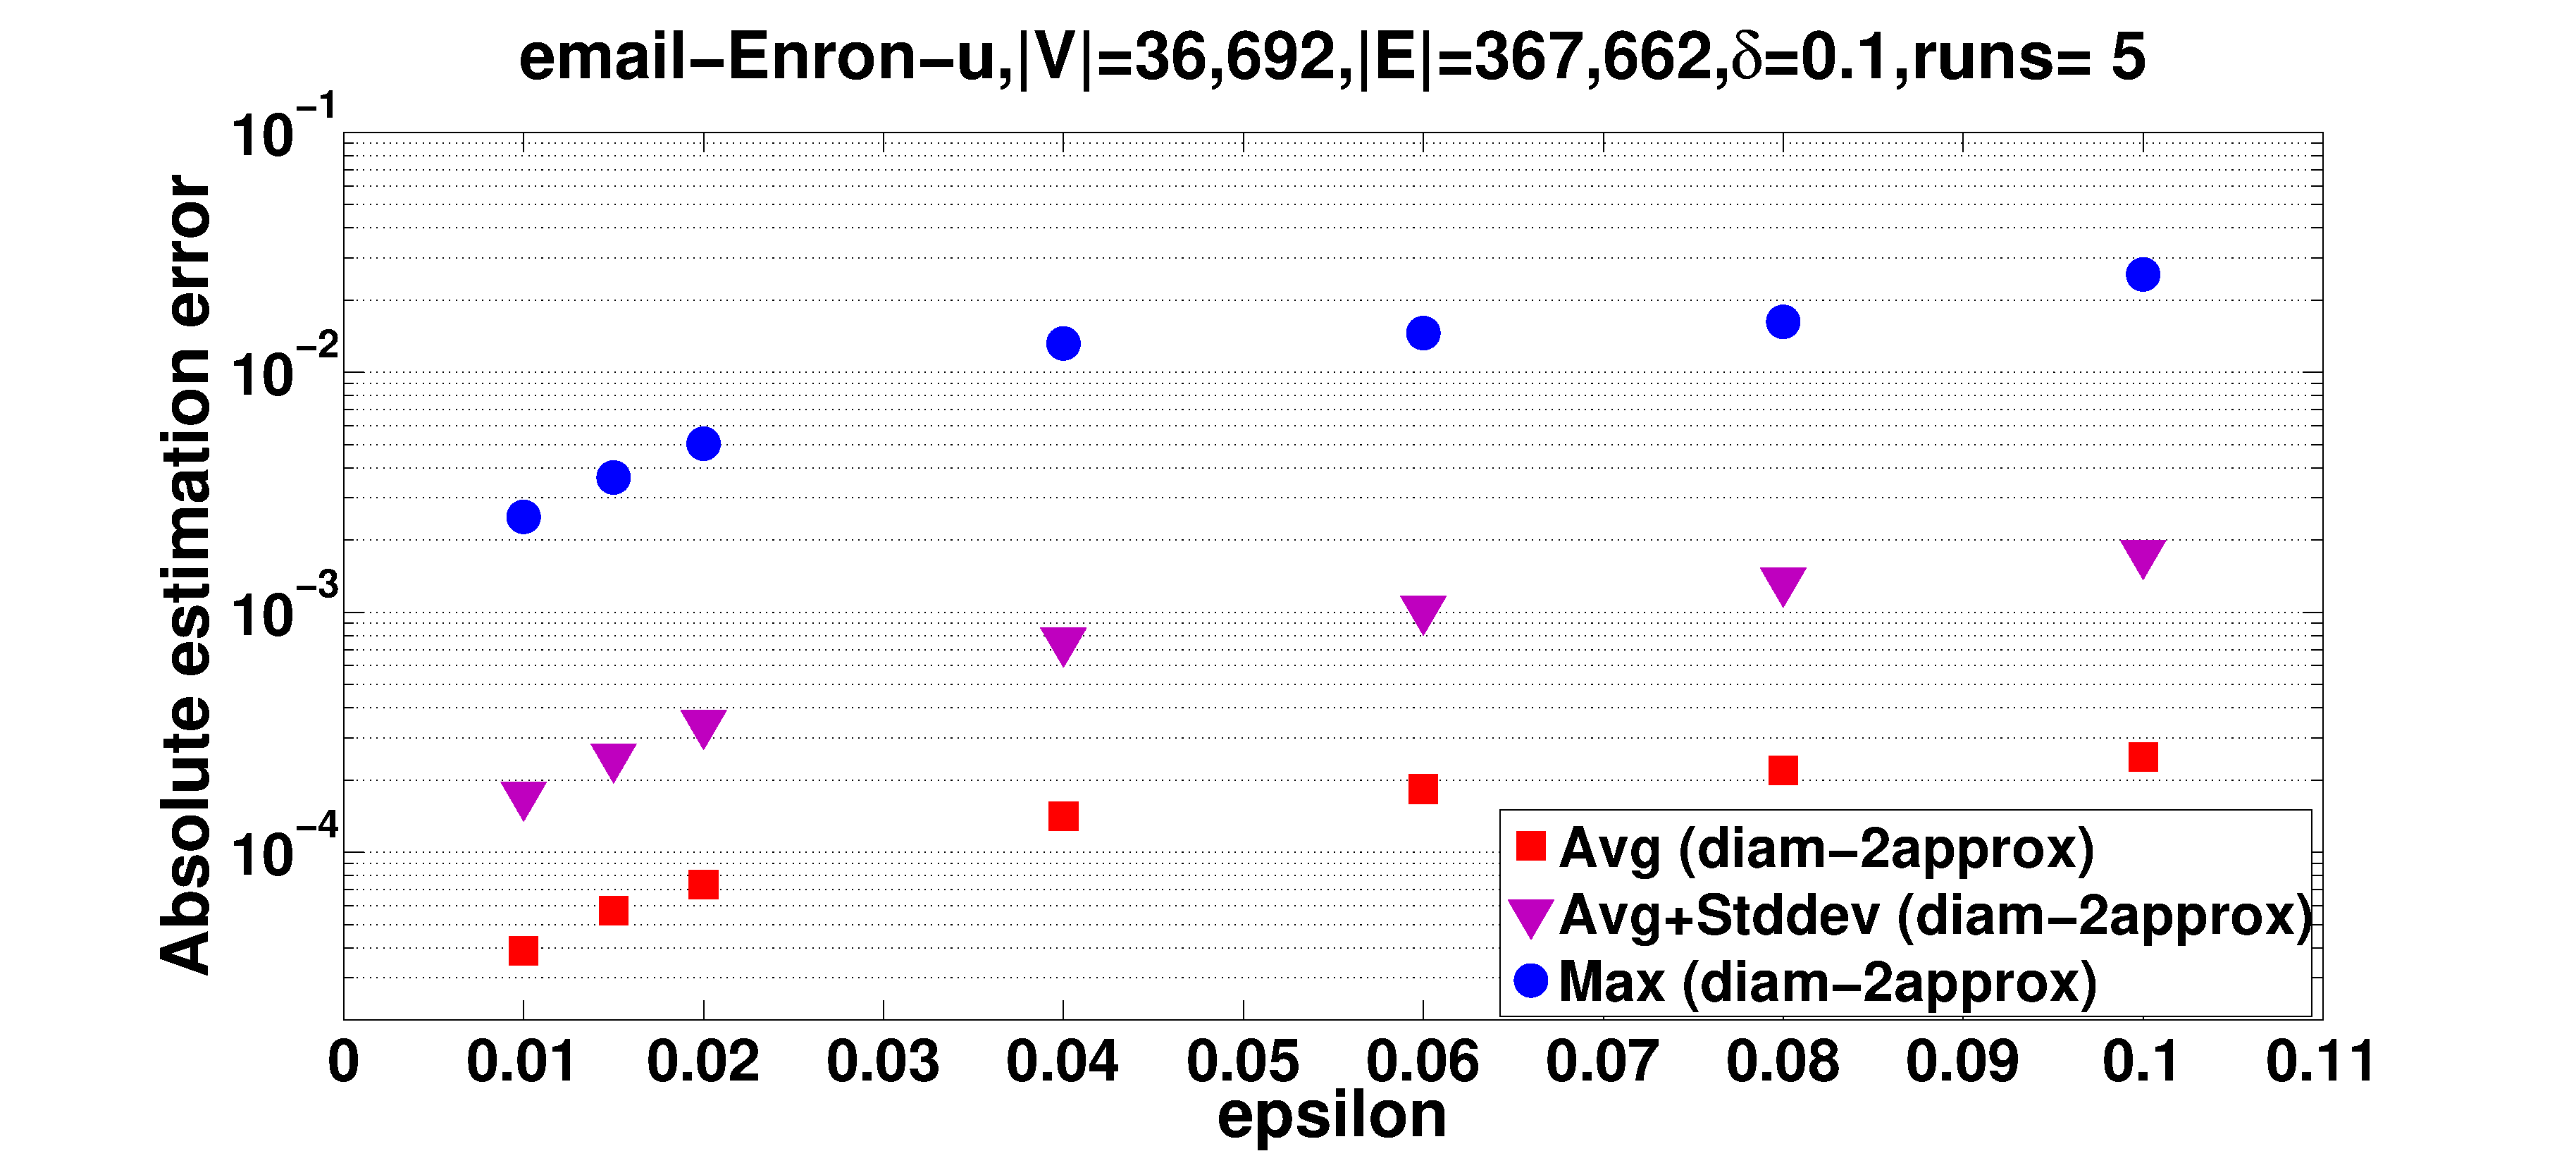
\includegraphics[scale=0.22]{figs/email-Enron-error}
  \end{figure}
\end{frame}

\begin{frame}
  \frametitle{How fast is the algorithm?}
  Approximately 8 times faster than the simple sampling algorithm
  \vfill
  Variable speedup w.r.t. exact algorithm (200x -- 4x), depending on
  $\varepsilon$
  \vfill
  \begin{figure}[H]
    \centering
    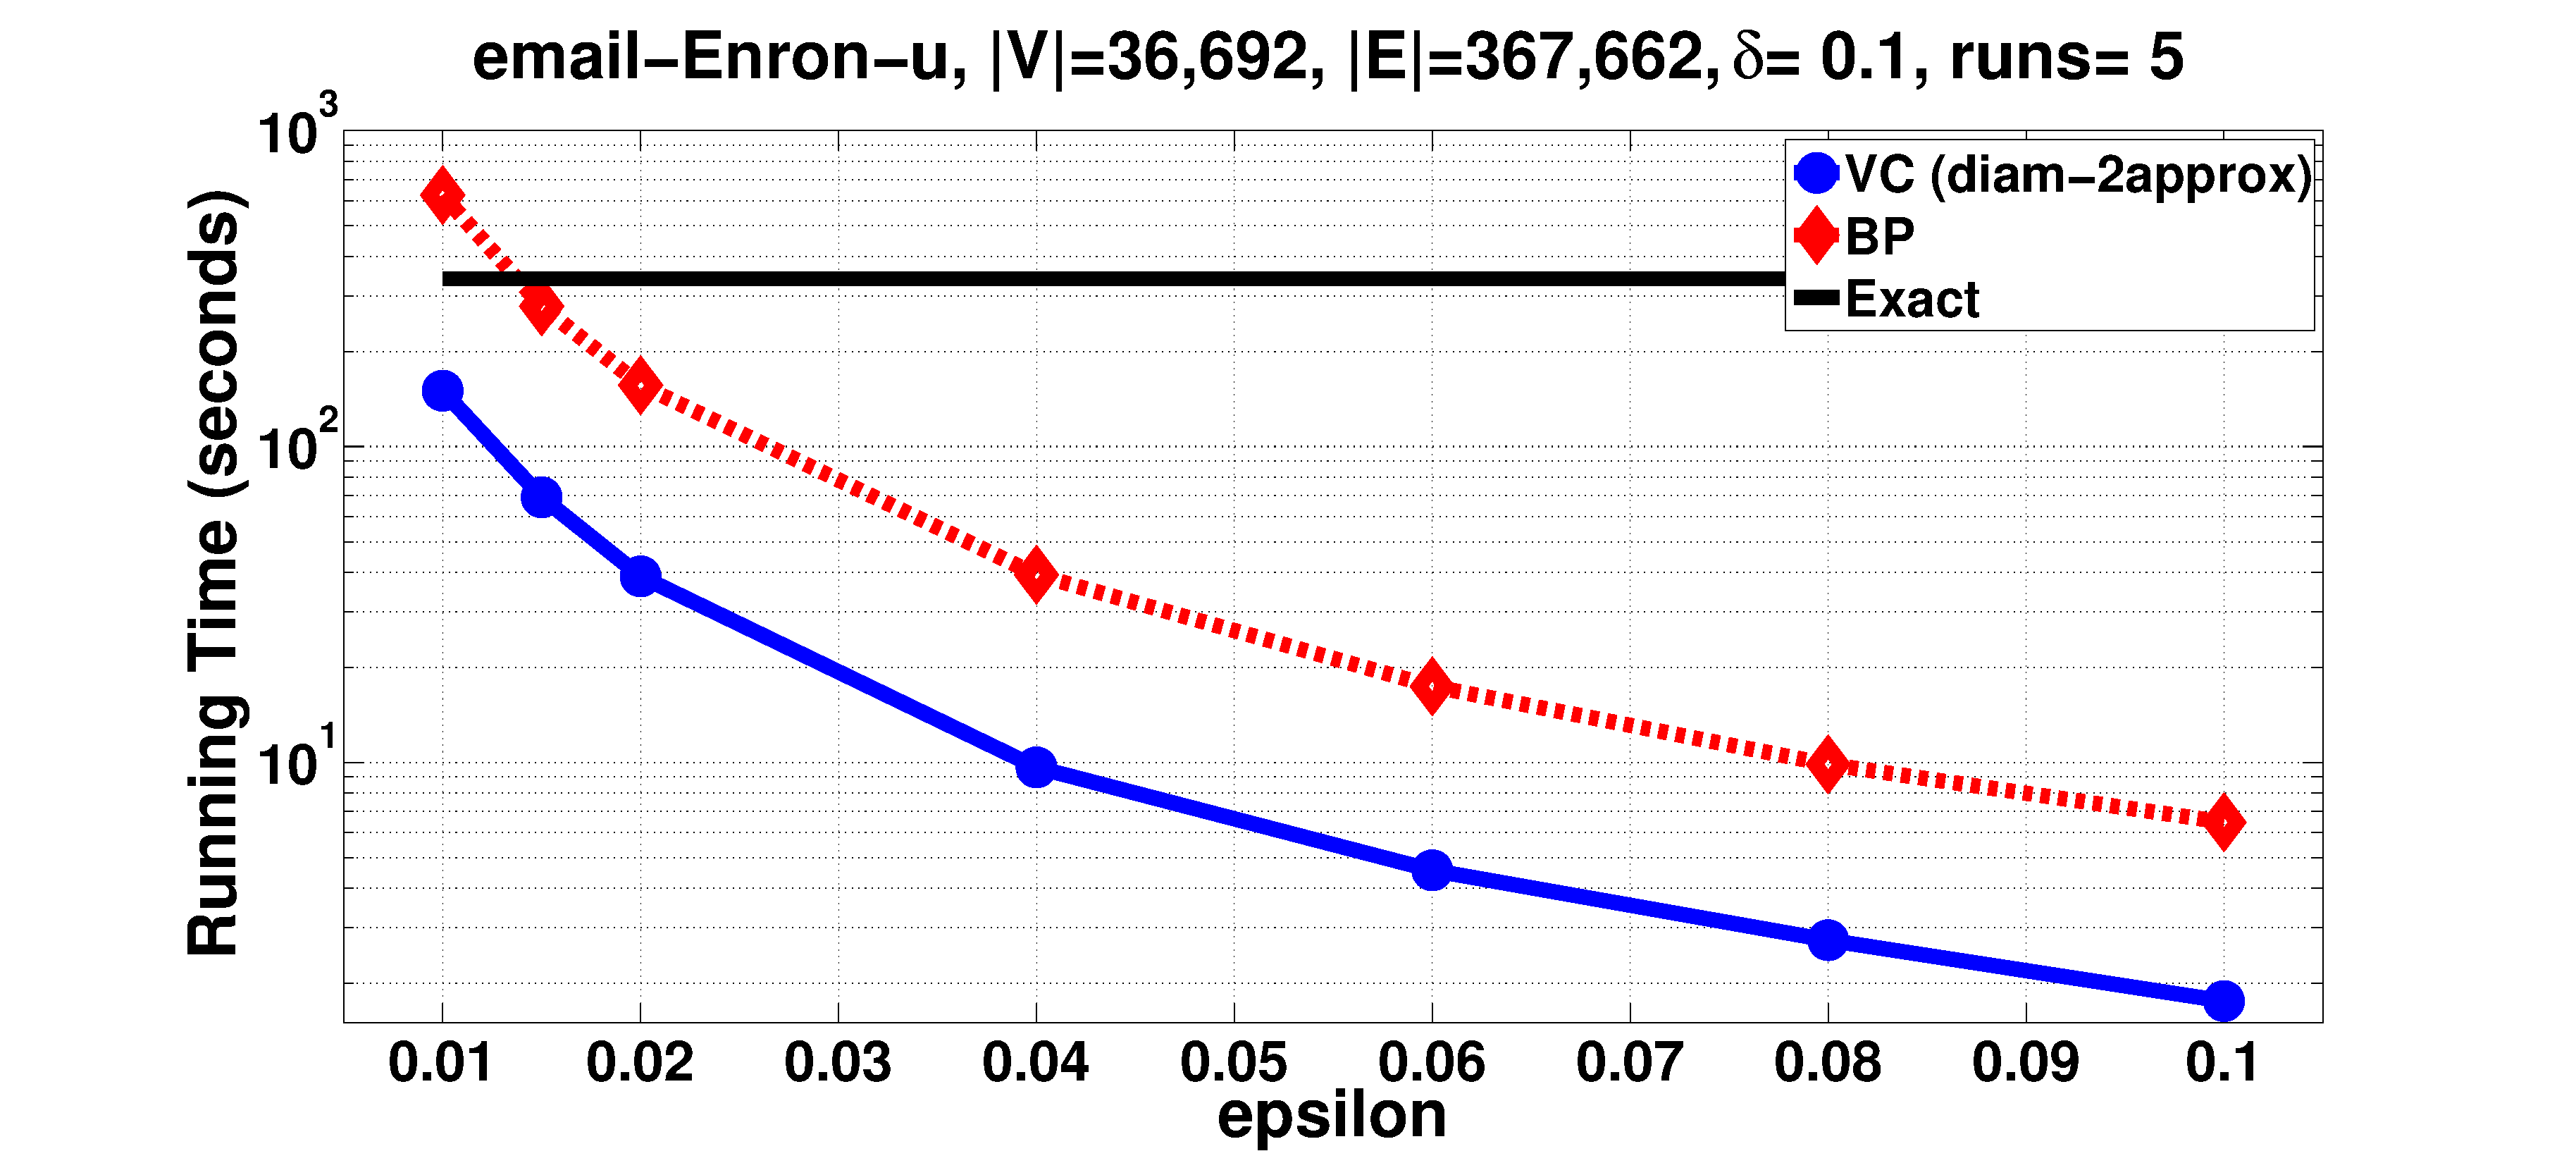
\includegraphics[scale=0.22]{figs/email-Enron-time}
  \end{figure}
\end{frame}

\begin{frame}
  \frametitle{How scalable is the algorithm?}
  Much more scalable than the simple sampling algorithm, because the sample
  size does not depend on $n$
  \vfill
  \begin{figure}[H]
    \centering
    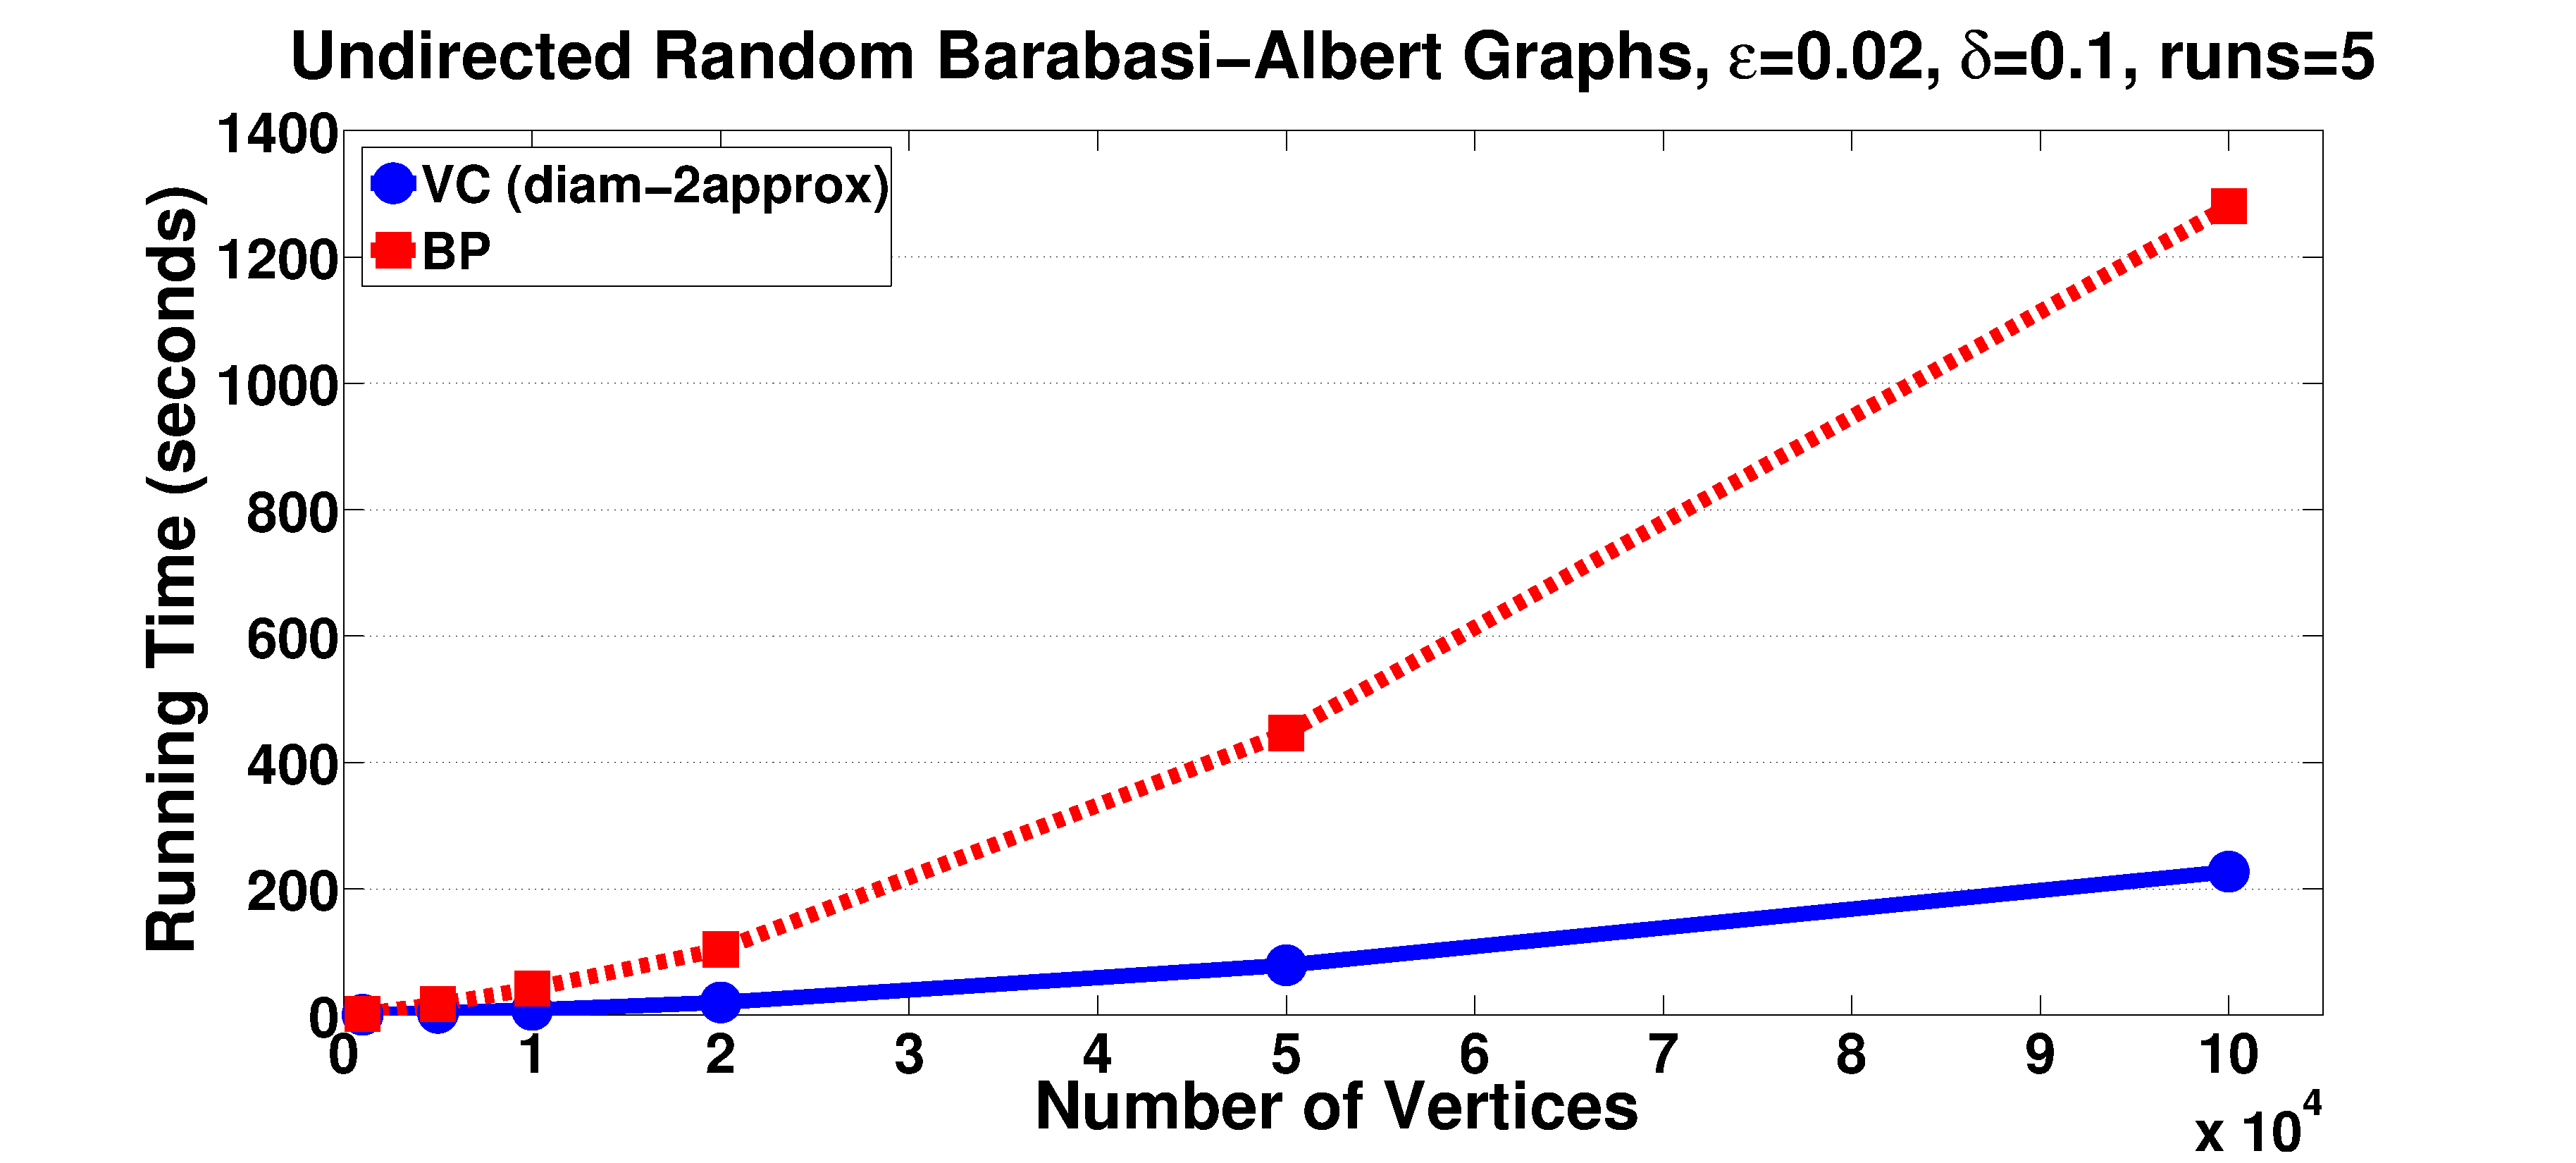
\includegraphics[scale=0.22]{figs/random-time}
  \end{figure}
\end{frame}

\begin{frame}
  \frametitle{Conclusions (Betweenness Centrality)}
  \vfill
  We showed a sampling algorithm for betweenness centrality approximation that
  gives probabilistic guarantees on the quality of the approximation for all
  the vertices
  \vfill
  The algorithm samples SPs according to a well-defined distribution, and
  the analysis relies on VC-dimension, which is bounded by the Vertex Diameter,
  a characteristic quantity of the graph that is small in real networks
  \vfill
  The use of VC-dimension makes the algorithm much faster and more scalable
  than previous sampling approaches and than the exact algorithm
\end{frame}

% !TEX root =  centrtutorial.tex
\begin{frame}
  \frametitle{Betweenness Centrality ? Incremental and Faster}
  \centering
  \vfill
  {\huge Meghana Nasre, Matteo Pontecorvi, Vijaya Ramachandran}
  \vfill
  {\large MFCS '14: Mathematical Foundations of Computer Science}
\end{frame}

\begin{frame}
  \frametitle{Path Dependency}
  
  \begin{itemize}
    \item Pair dependency of $(s,w)$ on $v$:
      \[\dep_{st}(w)=\frac{\paths_{sw}(v)}{\paths_{sw}}\]
    \item Dependency of a node $s$ on another node $v$:
      \[\dep_s(v)=\sum_{t \in V}\dep_{st}(w)\]
    \item Can be computed recursively:
    \[
    \dep_s(v)=\sum_{w \mid v \in \pred_s(w) } \frac{\paths_{sv}}{\paths_{sw}} \left( 1 + \dep_{s}(w) \right)
    \]
    \item Betweenness can be expressed as function of dependencies:
      \[ \betw(v) = \sum_{s \neq v} \dep_s(v) \]
  \end{itemize}
  
  \begin{figure}[H]
    \centering
    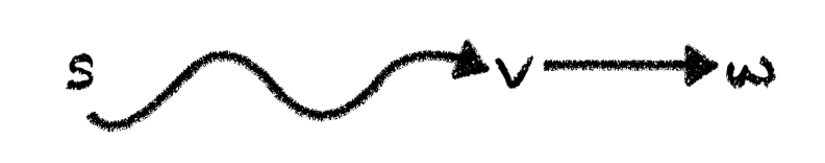
\includegraphics[scale=1]{imgs/path-dependency}
  \end{figure}
  
\end{frame}

\begin{frame}
  \frametitle{Main Result}

  \begin{figure}[H]
    \centering
    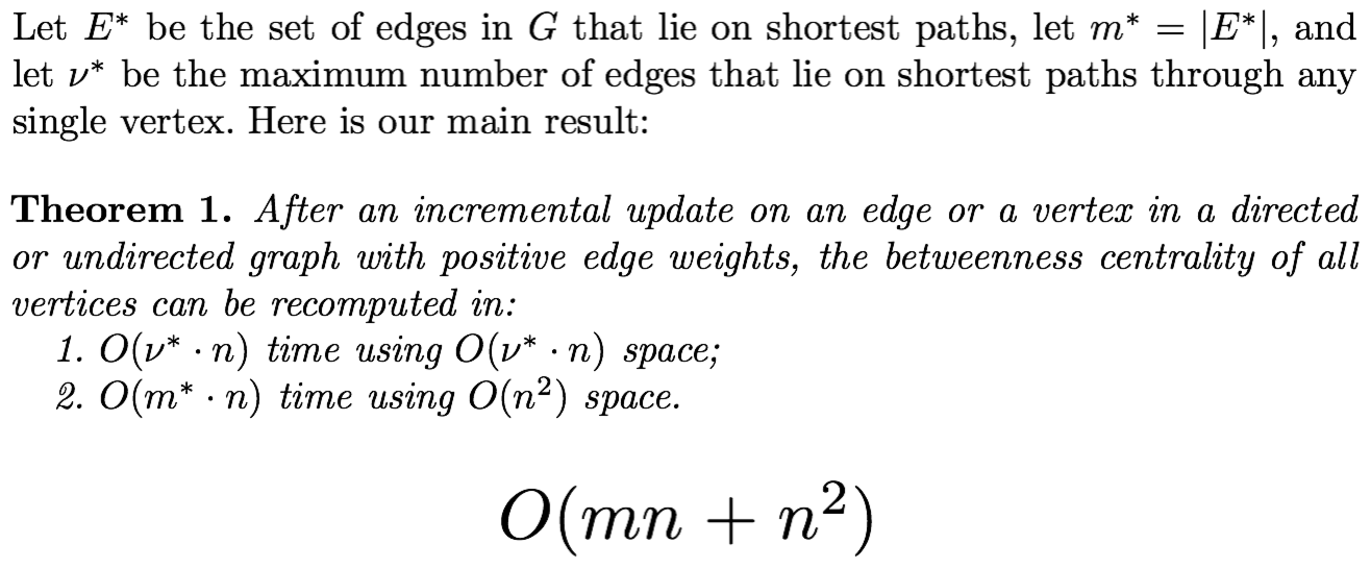
\includegraphics[width=\textwidth]{imgs/npr14-main-result}
  \end{figure}
  
\end{frame}

\begin{frame}
  \frametitle{Lemmas}

  \begin{figure}[H]
    \centering
    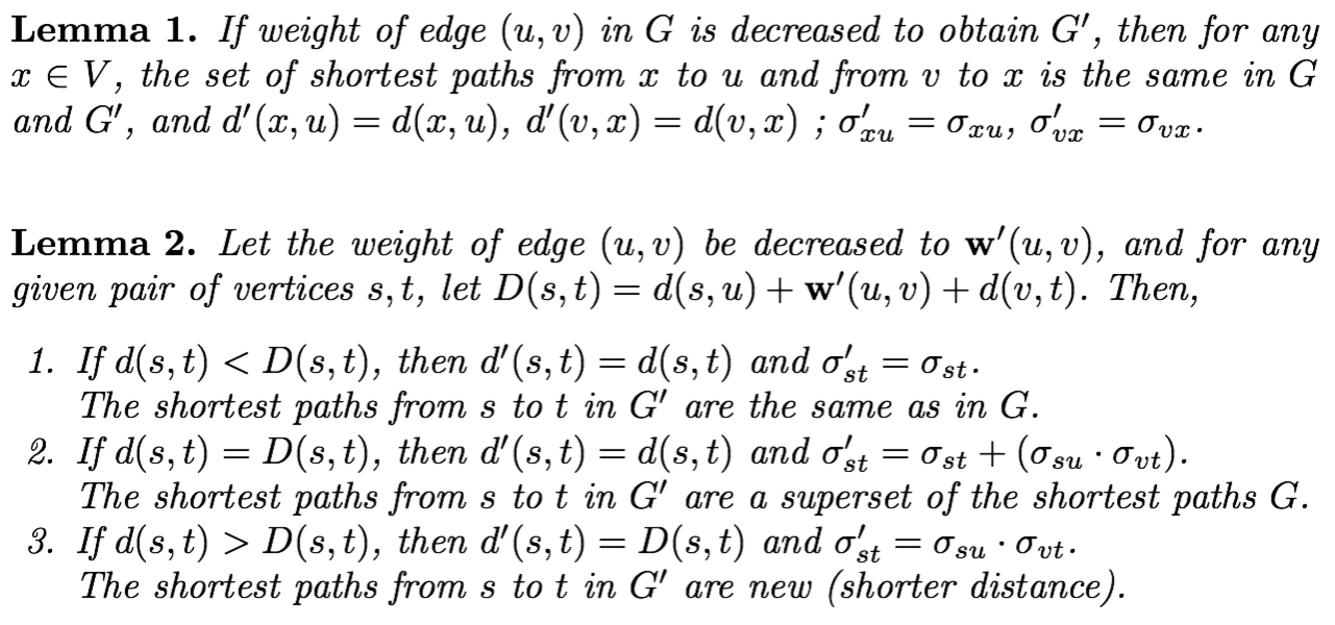
\includegraphics[width=\textwidth]{imgs/npr14-lemmas}
  \end{figure}
  
\end{frame}

\begin{frame}
  \frametitle{SSSP DAG Update}

  \begin{figure}[H]
    \centering
    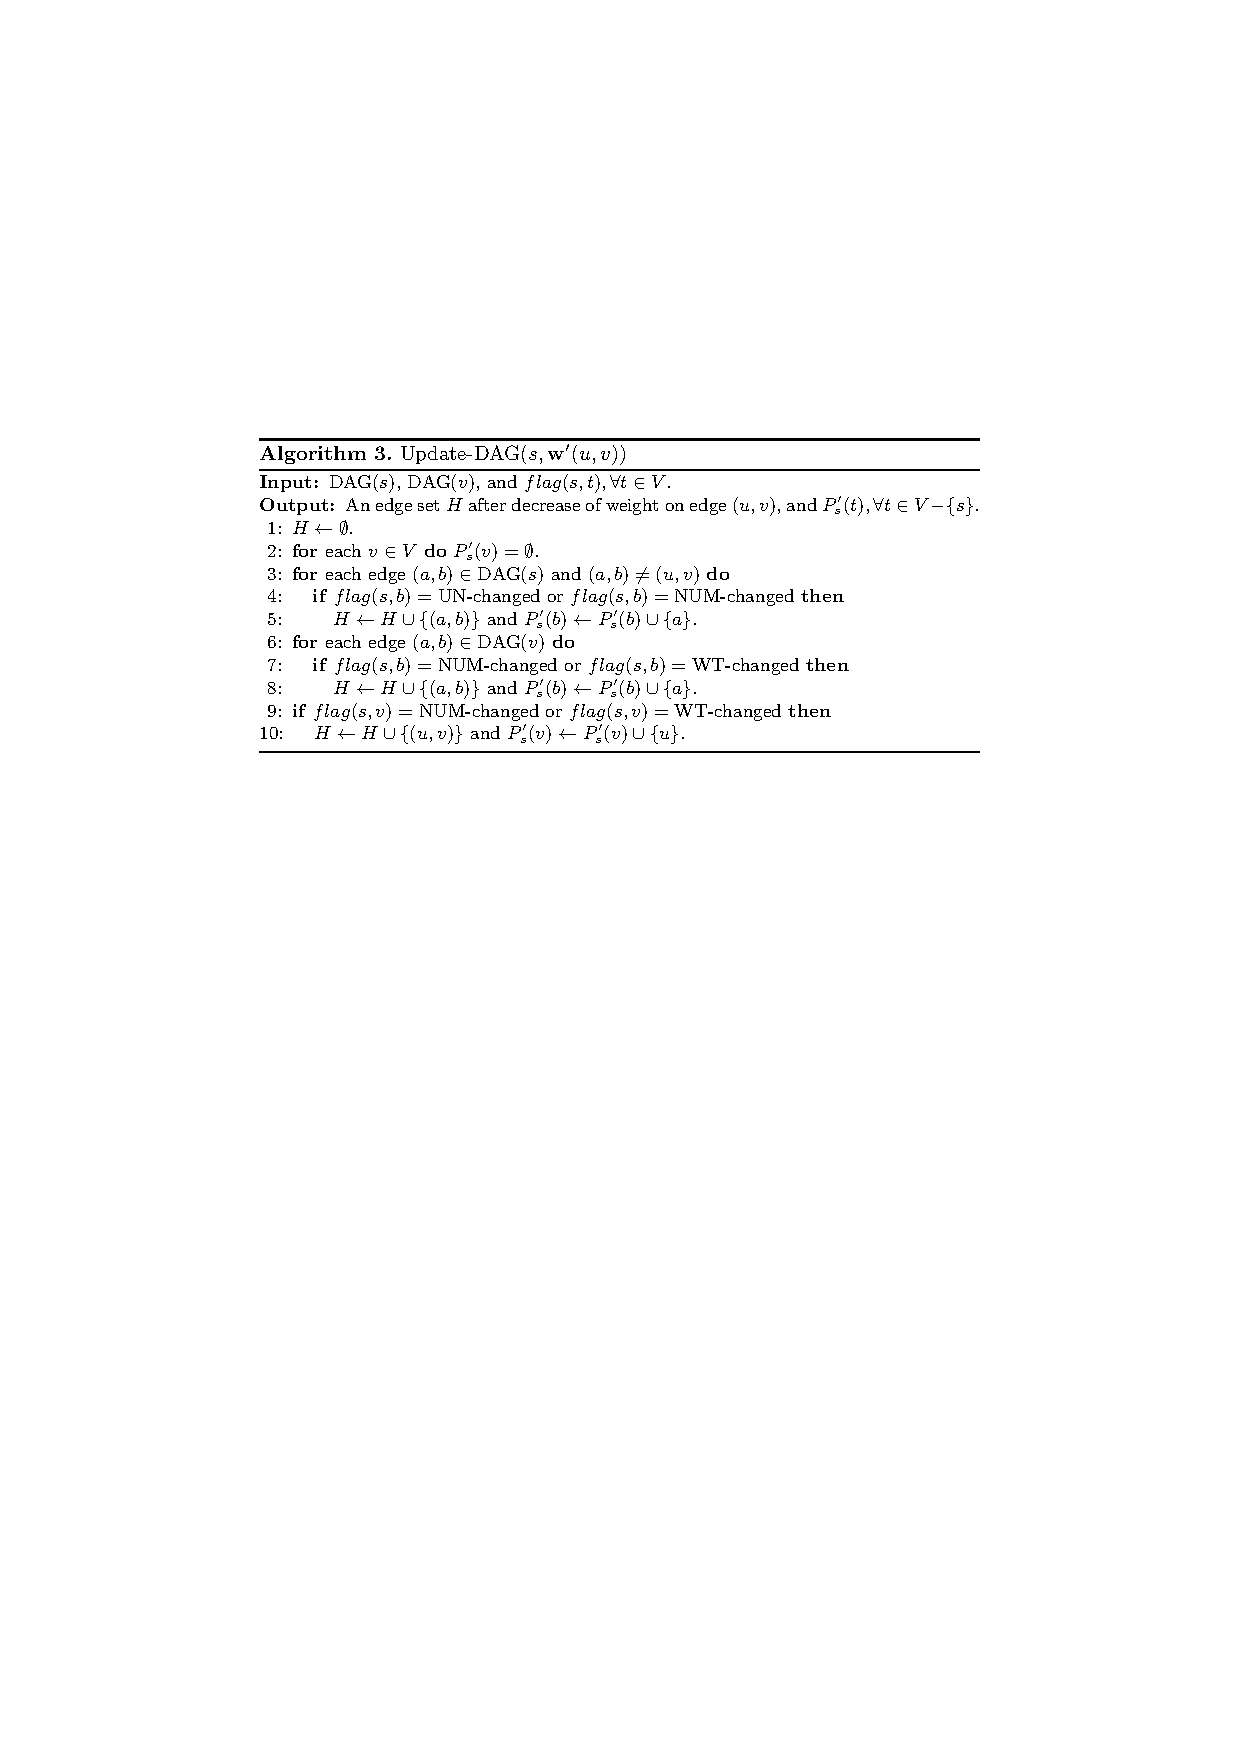
\includegraphics[width=\textwidth]{imgs/npr14-algo3}
  \end{figure}
  
\end{frame}

\begin{frame}
  \frametitle{Edge Update}

  \begin{figure}[H]
    \centering
    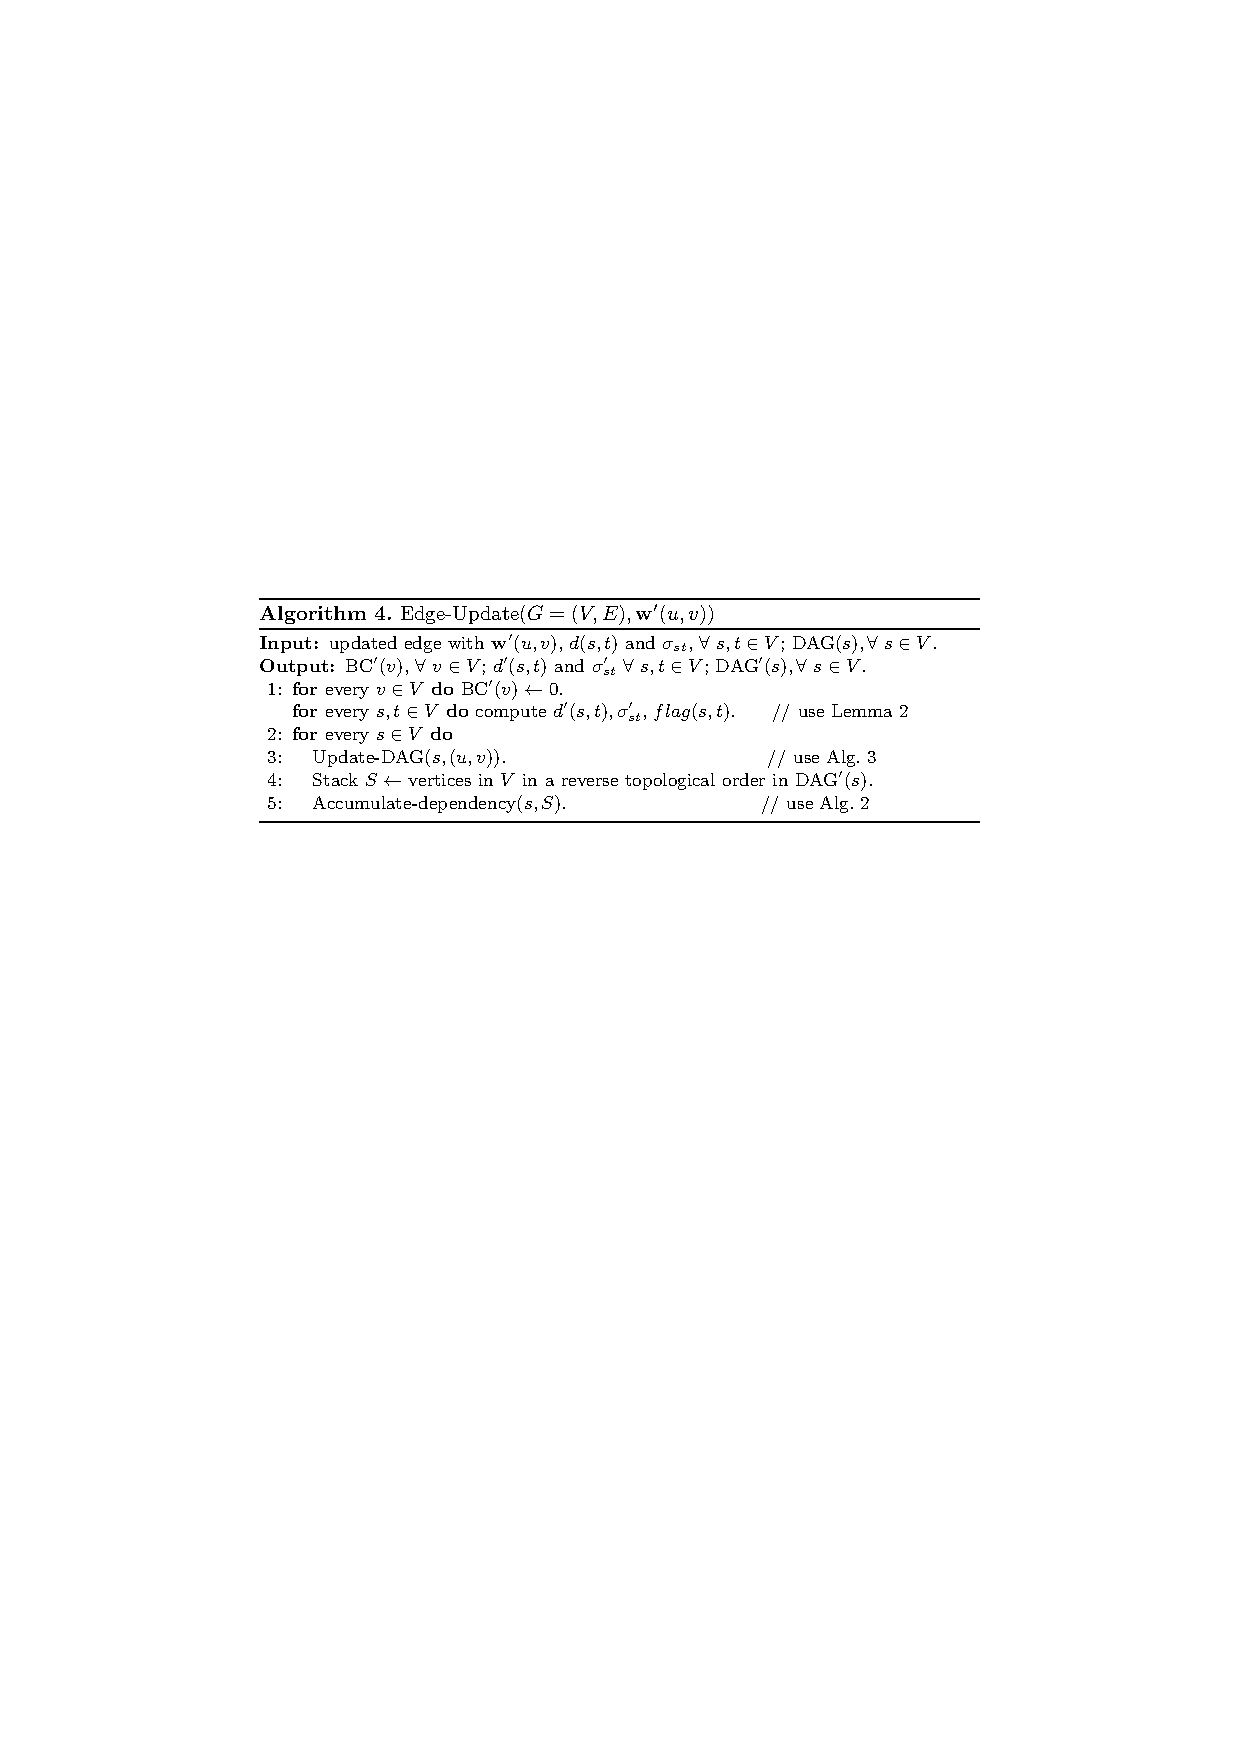
\includegraphics[width=\textwidth]{imgs/npr14-algo4}
  \end{figure}
  
\end{frame}

\begin{frame}
  \frametitle{Space-Efficient Variant $O(n^2)$}
  
  \begin{itemize}
    \item Do not store the \sssp \dag
    \item Store only $E^*$
    \item Updated \dag can be build in $O(m^*)$ time
    \begin{itemize}
      \item Time $O(m^* \times n)$
      \item Compute ${E'}^*$ from $E^*$, then $\dag'(s)$ from ${E'}^*$
    \end{itemize}
    \item Space $O(m^* + n^2)$ to store $E^*$ and $n^2$ distances $\dist(s,t)$ and shortest paths $\paths_{st}$
  \end{itemize}
  
\end{frame}

\begin{frame}
  \frametitle{Comparison}

  \begin{figure}[H]
    \centering
    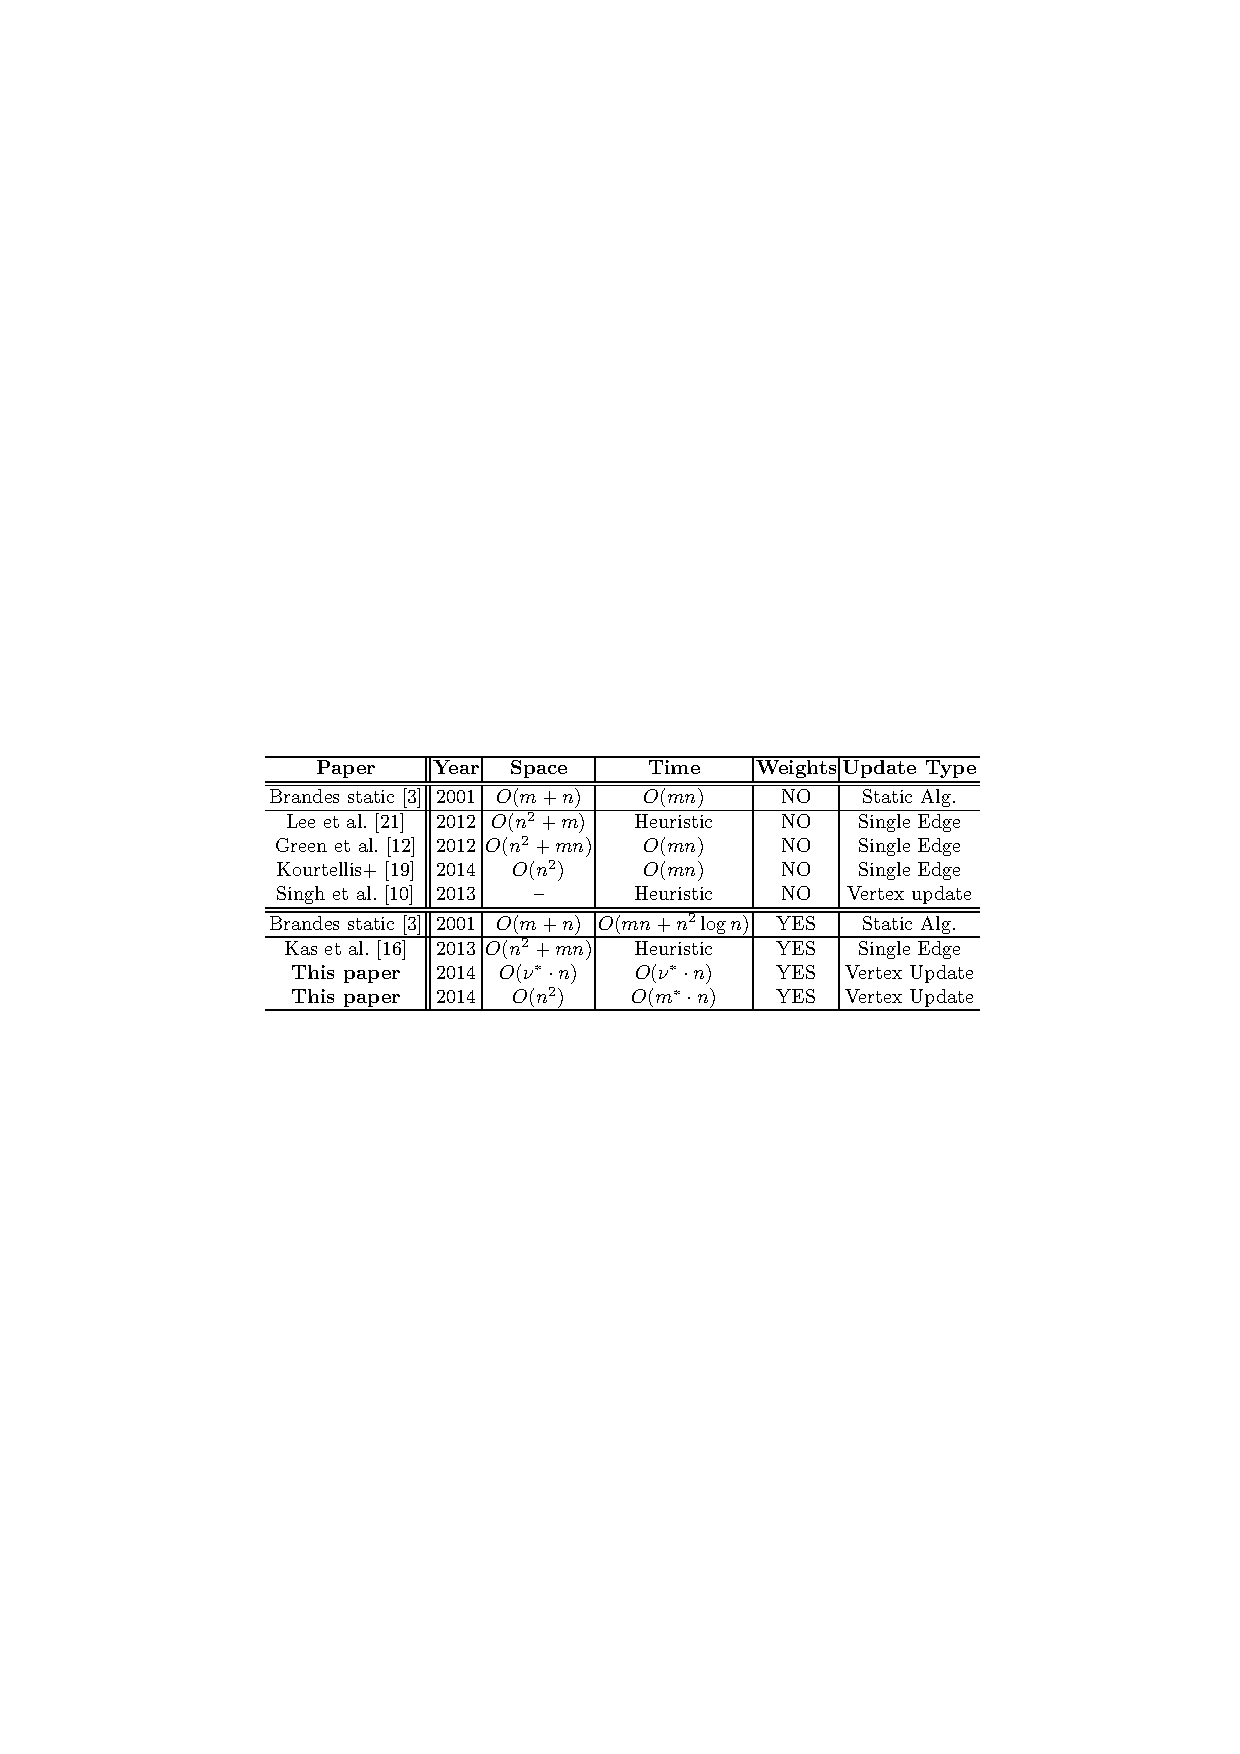
\includegraphics[width=\textwidth]{imgs/npr14-comparison}
  \end{figure}
  
\end{frame}

\begin{frame}
  \frametitle{Shortcomings}

  \begin{itemize}
    \item Not fully dynamic (no edge removal)
    \item $m^*$ can be large in practice
    \item Non-trivial to parallelize (need to access pairs of \sssp \dag at a time)
    \item Does not solve main bottleneck of most algorithms: $O(n^2)$ memory
  \end{itemize}
  
\end{frame}

% !TEX root =  centrtutorial.tex

\begin{frame}
  \frametitle{Part 4}
  \centering
  \Huge Scalable Dynamic Algorithms
\end{frame}


\begin{frame}
  \frametitle{Parallelism}

  \begin{itemize}
    \item Fine grained: single concurrent BFS
    \item Only one copy of auxiliary data structires
    \item Synchronization needed
    \item Better for GPUs, which have small memory
  \end{itemize}
  \begin{itemize}
    \item Coarse grained: many independent BFSs
    \item Sources are independent, embarrassingly parallel
    \item More memory needed
    \item Better for CPUs, which have large memory
  \end{itemize}
\end{frame}
 
 
%% Sariy�ce et al.
\begin{frame}
  \frametitle{Betweenness Centrality on GPUs and Heterogeneous Architectures}
  \centering
  \vfill
  {\huge A. E. Sariy�ce, K. Kaya, E. Saule, �.~V.~�ataly�rek}
  \vfill
  {\large GPGPU '13: Workshop on General Purpose Processing Using GPUs}
\end{frame}


\begin{frame}
  \frametitle{GPU}

  \begin{quote}
    A GPU is especially well-suited to address problems that can be expressed as \textbf{data-parallel computations} - the same program is executed on many data elements in parallel - with \textbf{high arithmetic intensity} - the ratio of arithmetic operations to memory operations.
    
    Because the same program is executed for each data element, there is a lower requirement for sophisticated flow control, and because it is executed on many data elements and has high arithmetic intensity, the memory access latency can be hidden with calculations instead of big data caches.\footnote{\url{http://docs.nvidia.com/cuda/cuda-c-programming-guide/index.html}}
  \end{quote}
\end{frame}


\begin{frame}
  \frametitle{Execution model}
  \begin{columns}[onlytextwidth]

    \begin{column}{0.5\textwidth}
      \begin{itemize}
        \item One thread per data element
        \item Thread scheduled in blocks with barriers (wait for others at the end)
        \item Program runs on the whole data (kernel)
      \end{itemize}
      \begin{itemize}
        \item Minimize synchronization
        \item Balance load
        \item Coalesce memory access
      \end{itemize}
    \end{column}

    \begin{column}{0.5\textwidth}
      \begin{figure}[t]
        \centering
        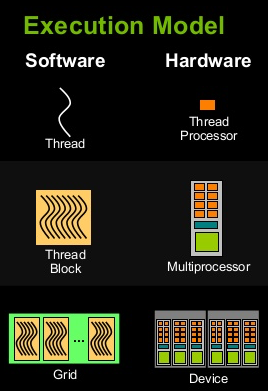
\includegraphics[width=\textwidth, height=0.8\textheight, keepaspectratio]{imgs/cuda}
      \end{figure}
    \end{column}
  \end{columns}
  
\end{frame}


\begin{frame}
  \frametitle{Intuition}

  \begin{itemize}
    \item GPUs have huge number of cores
    \item Use them to parallelize BFS
    \item One core per vertex, or one core per edge
    \item Vertex-based parallelism creates load imbalance for graphs with skewed degree distribution
    \item Edge-based parallelism requires high memory usage
  \end{itemize}
  \begin{itemize}
    \item Use vertex-based parallelism
    \item Reduce memory usage by removing predecessors lists
    \item Virtualize high-degree nodes to address load imbalance
  \end{itemize}
  
\end{frame}


\begin{frame}
  \frametitle{Difference}
  
  \begin{columns}[onlytextwidth]
    \begin{column}{0.5\textwidth}
      \begin{figure}[t]
        \centering
        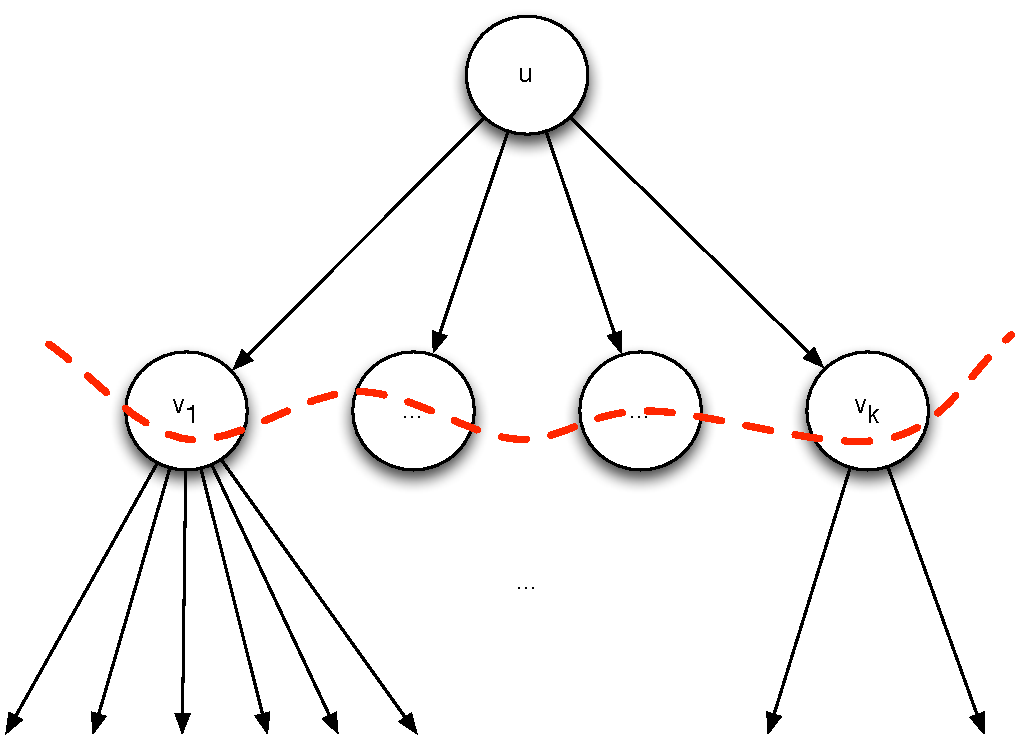
\includegraphics[width=\textwidth, height=0.6\textheight, keepaspectratio]{imgs/gpu-vertex-bfs}
        \caption{Vertex-based BFS}
      \end{figure}
    \end{column}
    
    \begin{column}{0.5\textwidth}
      \begin{figure}[t]
        \centering
        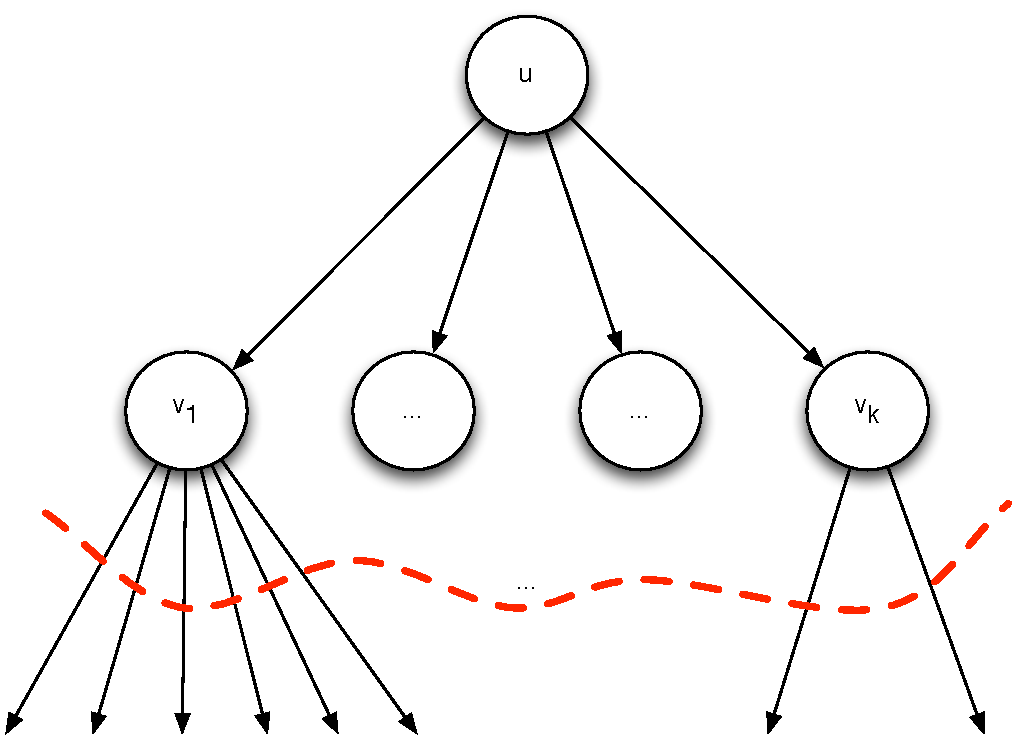
\includegraphics[width=\textwidth, height=0.6\textheight, keepaspectratio]{imgs/gpu-edge-bfs}
        \caption{Edge-based BFS}
      \end{figure}
    \end{column}
  \end{columns}

\end{frame}


\begin{frame}
  \frametitle{Vertex-based}
  
  \begin{columns}[onlytextwidth]
    \begin{column}{0.5\textwidth}
      \begin{itemize}
        \item For each level, for each vertex in parallel
        \item If vertex is on level
        \item For each neighbor, adjust \pred and \paths
        \item Atomic update on \paths needed (multiple paths can be discovered concurrently)
        \item While backtracking, if $u \in \pred(v)$ accumulate $\dep(u) = \dep(u) + \dep(v)$
        \item Possible load imbalance if degree skewed
      \end{itemize}
    \end{column}

    \begin{column}{0.5\textwidth}
      \begin{figure}[t]
        \centering
        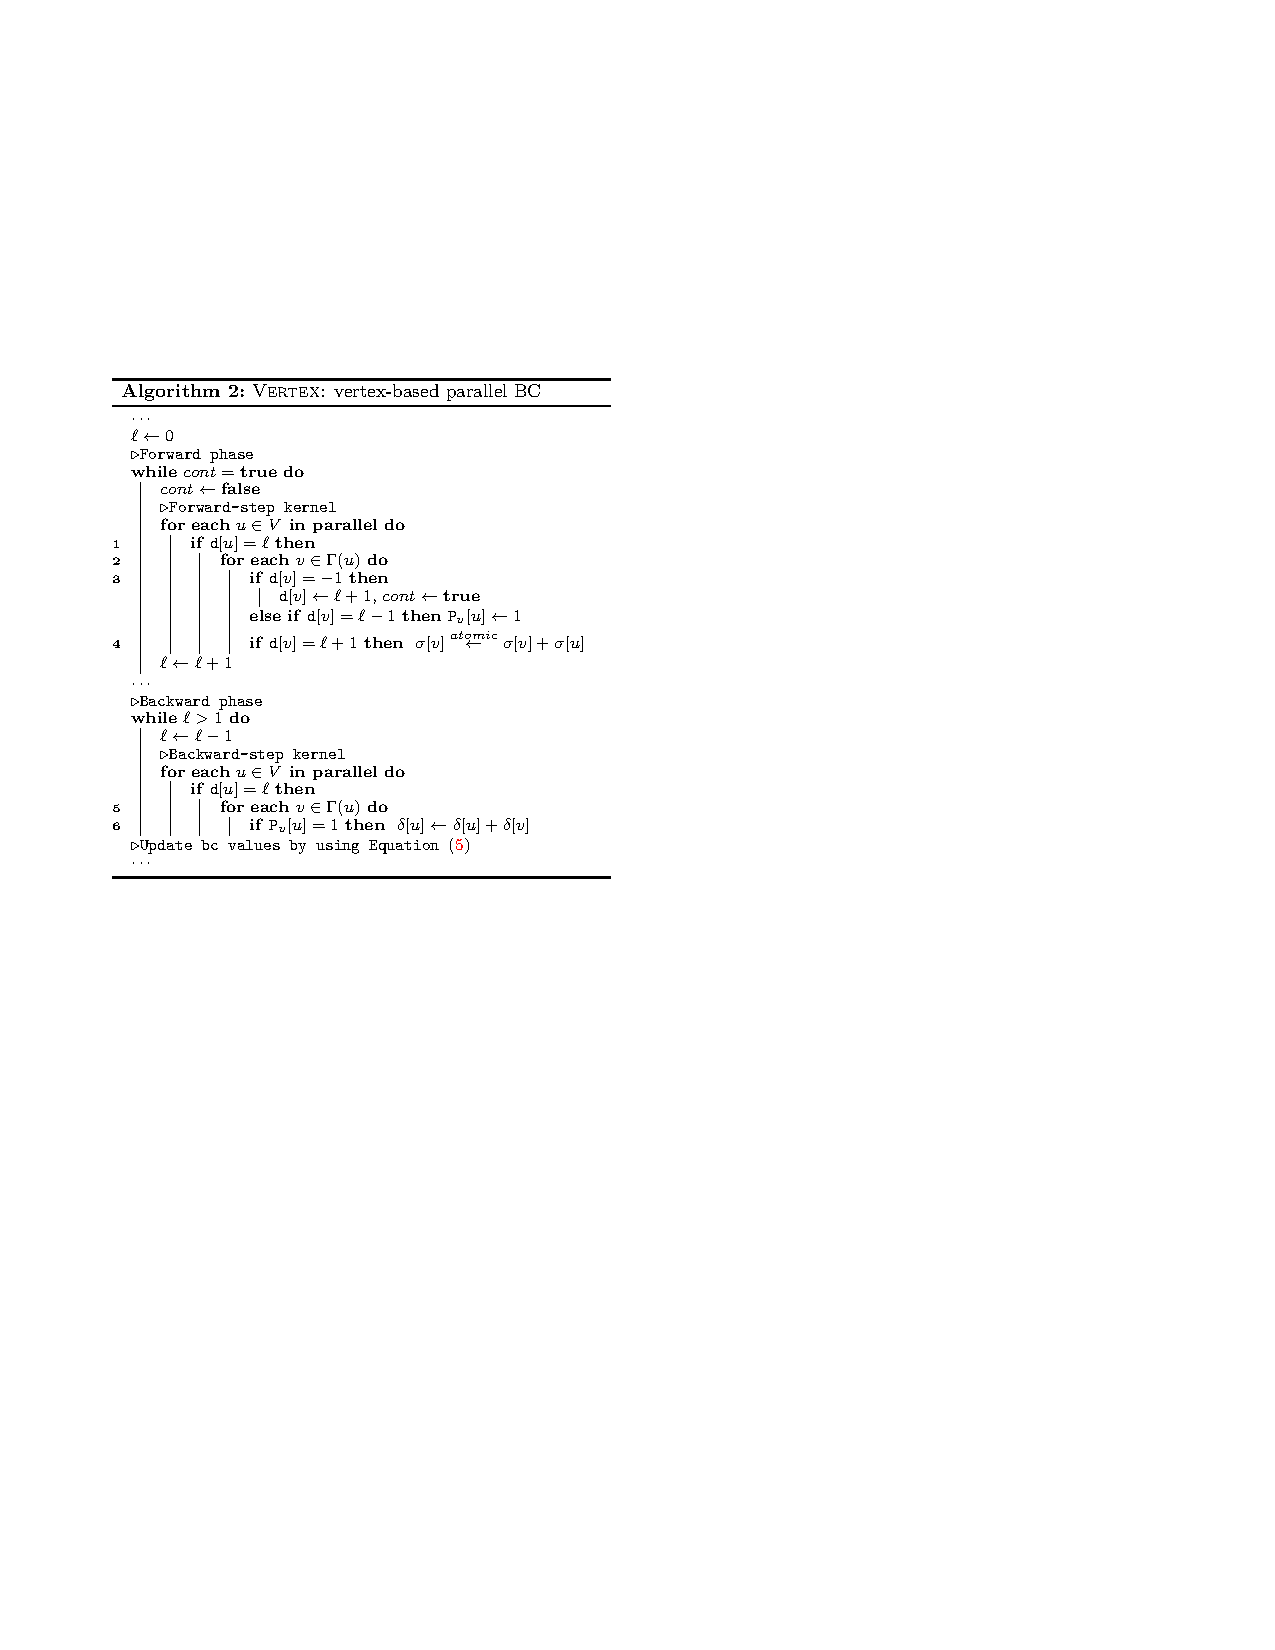
\includegraphics[width=\textwidth, height=0.8\textheight, keepaspectratio]{imgs/gpu-algo-vertex}
      \end{figure}
    \end{column}
  \end{columns}
  
\end{frame}


\begin{frame}
  \frametitle{Edge-based}
  
  \begin{columns}[onlytextwidth]
    \begin{column}{0.5\textwidth}
      \begin{itemize}
        \item For each level, for each edge in parallel
        \item If edge endpoint is on level
        \item Same as above...
        \item While backtracking, if $u \in \pred(v)$ accumulate $\dep(u) = \dep(u) + \dep(v)$ \emph{atomically}
        \item Multiple edges can try to update \dep concurrently
        \item More memory (edge-based layout) \\ and more atomic operations
      \end{itemize}
    \end{column}

    \begin{column}{0.5\textwidth}
      \begin{figure}[t]
        \centering
        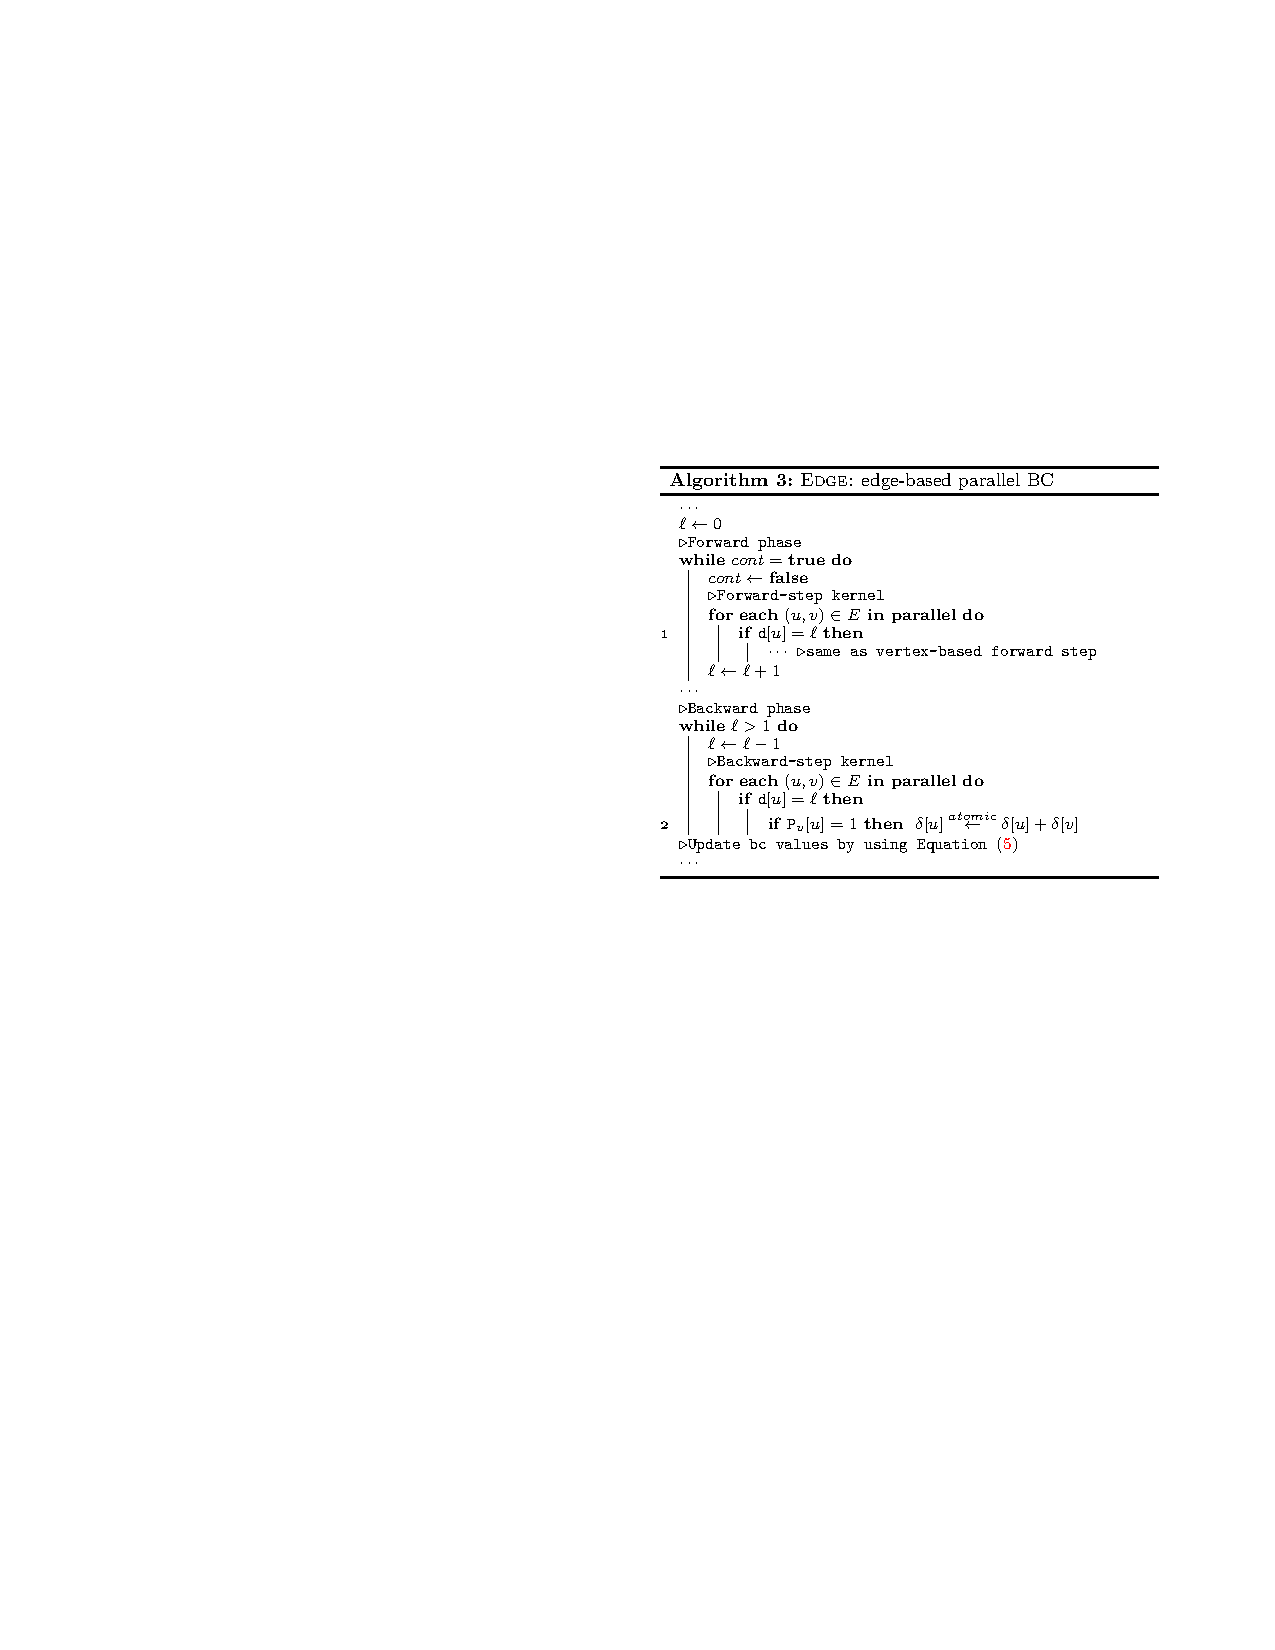
\includegraphics[width=\textwidth, height=0.8\textheight, keepaspectratio]{imgs/gpu-algo-edge}
      \end{figure}
    \end{column}
  \end{columns}
  
\end{frame}


\begin{frame}
  \frametitle{Vertex virtualization}

  \begin{columns}[onlytextwidth]
    \begin{column}{0.5\textwidth}
      \begin{itemize}
        \item AKA, edge packing/batching, \\ hybrid between vertex- and edge-based
        \item Split high degree vertices into virtual ones with maximum degree $mdeg$
        \item Equivalently, pack up to $mdeg$ edges belonging to the same vertex together
        \item Very small $mdeg = 4$
        \item Need additional auxiliary maps
      \end{itemize}
    \end{column}

    \begin{column}{0.5\textwidth}
      \begin{figure}[t]
        \centering
        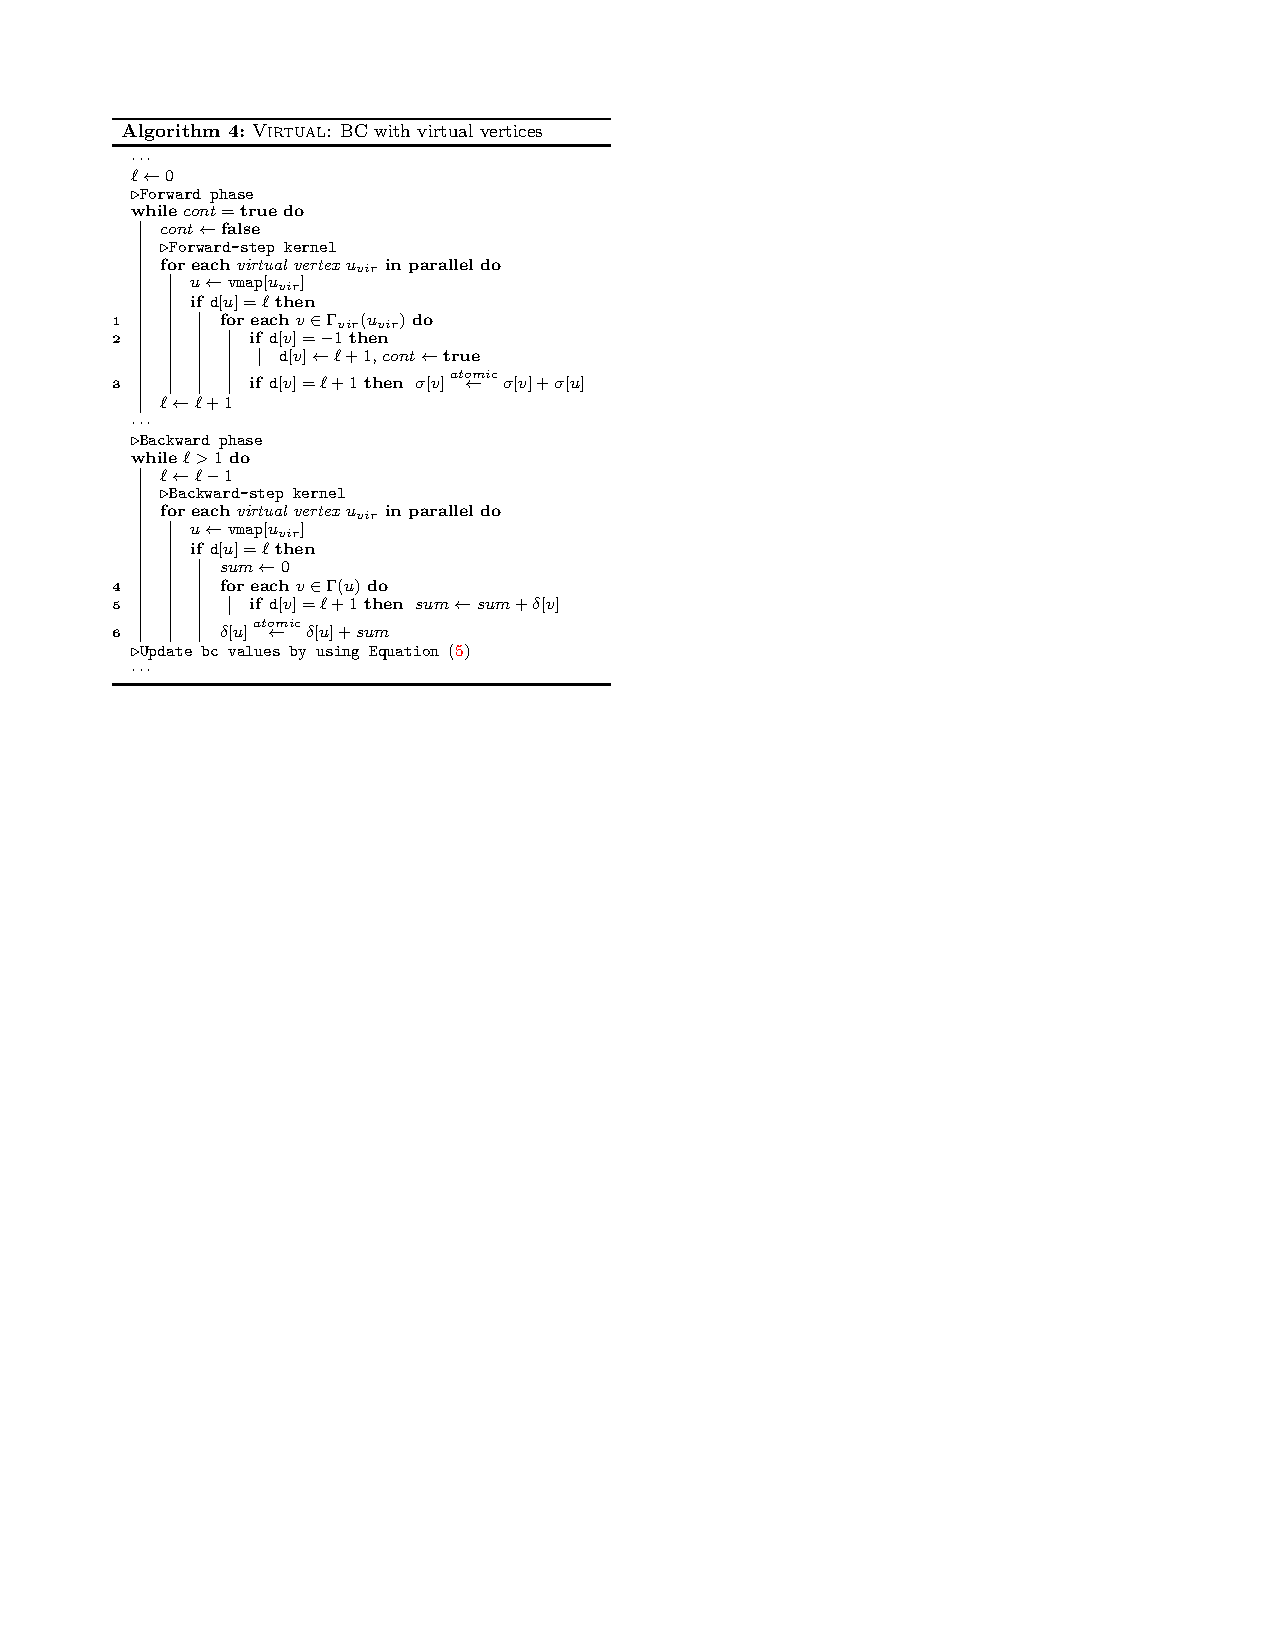
\includegraphics[width=\textwidth, height=0.8\textheight, keepaspectratio]{imgs/gpu-algo-hybrid}
      \end{figure}
    \end{column}
  \end{columns}
  
\end{frame}


\begin{frame}
  \frametitle{Benefits}
  
  \begin{itemize}
    \item Compared to vertex-based:
    \begin{itemize}
      \item Reduce load imbalance
    \end{itemize}
    \item Compared to edge-based:
    \begin{itemize}
    \item Reduce number of atomic operations
    \item Reduce memory footprint
    \end{itemize}
    \item Predecessors stored implicitly in the \spdag level (reduced memory usage)
    \item Memory layout can be further optimized to coalesce latency via \emph{striding}:
    \begin{itemize}
      \item Distribute edges to virtual vertices in round-robin
      \item When accessed in parallel, they create faster sequential memory access pattern
    \end{itemize}
  \end{itemize}
\end{frame}


\begin{frame}
  \frametitle{Results}

  \begin{figure}[t]
    \centering
    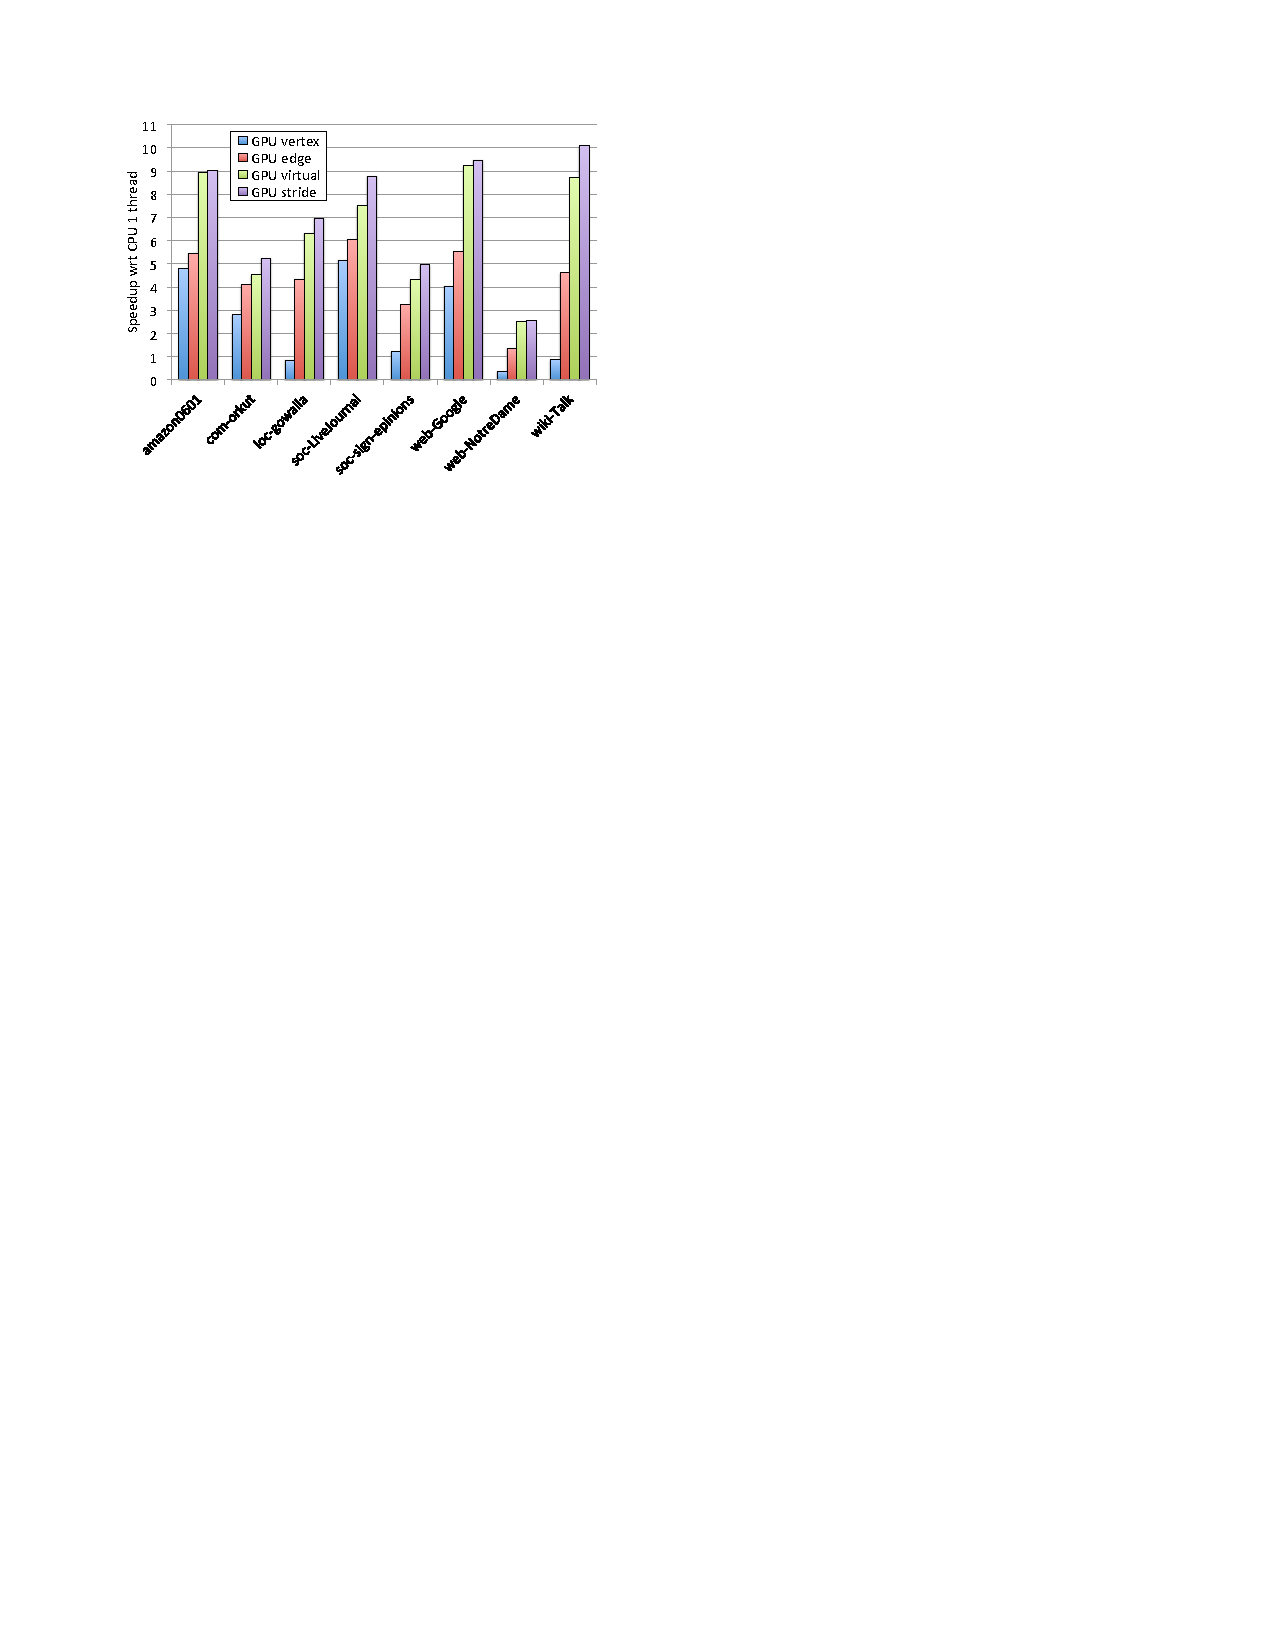
\includegraphics[width=\textwidth, height=0.6\textheight, keepaspectratio]{imgs/gpu-results1}
    \caption{Speedup}
  \end{figure}

  \begin{itemize}
    \item Results computed only on a sample of the graphs sources and extrapolated linearly
  \end{itemize}
\end{frame}


\begin{frame}
  \frametitle{Results}

  \begin{figure}[t]
    \centering
    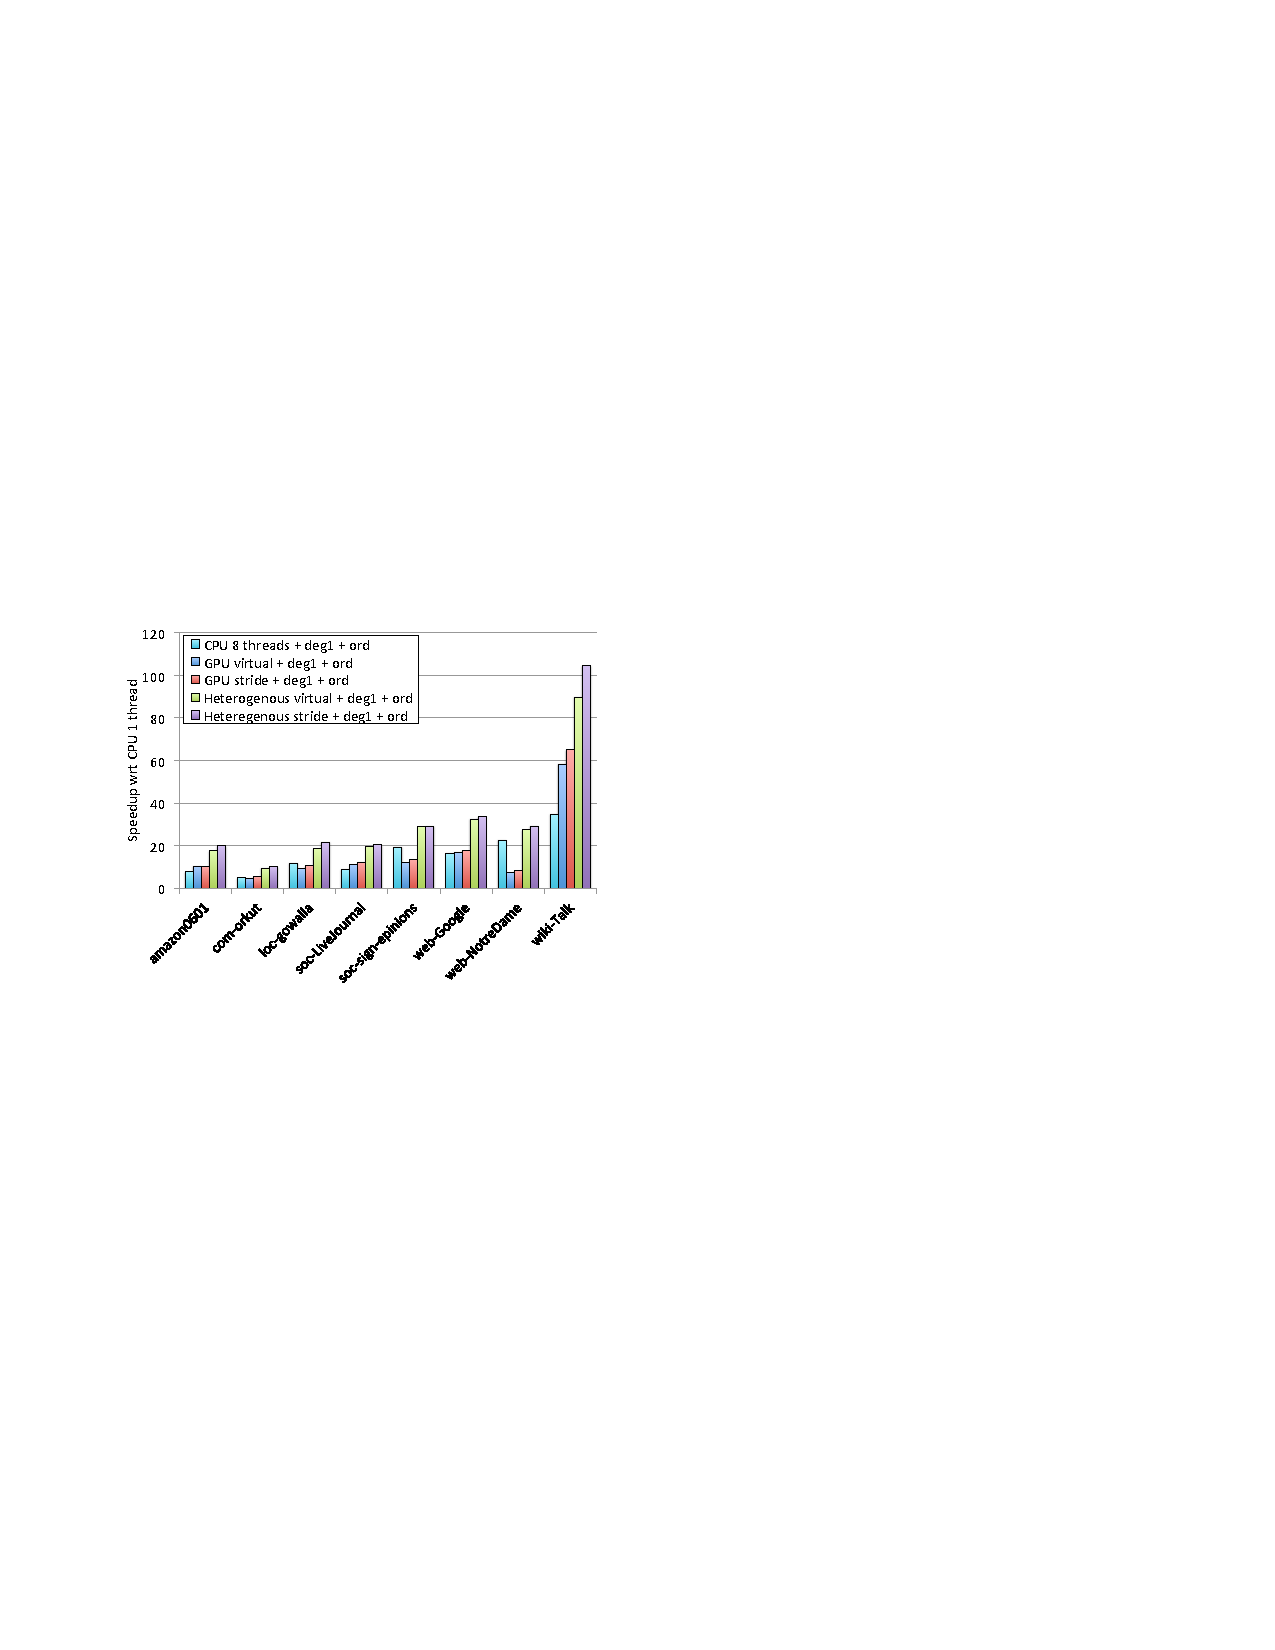
\includegraphics[width=\textwidth, height=0.6\textheight, keepaspectratio]{imgs/gpu-results2}
    \caption{Speedup}
  \end{figure}
    
\end{frame}


%% Kourtellis et al.
\begin{frame}
  \frametitle{Scalable Online Betweenness Centrality in Evolving Graphs}
  \centering
  \vfill
  {\huge N. Kourtellis, G. De-Francisci-Morales, F. Bonchi}
  \vfill
  {\large TKDE: IEEE Transactions on Knowledge and Data Engineering (2015)}
\end{frame}

\bibliographystyle{abbrvnat}
\bibliography{../proceedings/centrality.bib}

\end{document}
